\documentclass[cs4size,a4paper,10pt]{ctexart}   

\linespread{1.5}
\usepackage{geometry}%用于设置上下左右页边距
	\geometry{left=2.5cm,right=2.5cm,top=3.2cm,bottom=2.7cm}
\usepackage{xeCJK,amsmath,paralist,enumerate,booktabs,multirow,graphicx,subfig,setspace,listings,lastpage,hyperref}
\usepackage{amsthm, amssymb, bm, color, framed, graphicx, hyperref, mathrsfs}
\usepackage{mathrsfs}  
	\setlength{\parindent}{2em}
	\lstset{language=Matlab}%
\usepackage{fancyhdr}
\usepackage{graphicx}
\usepackage{subfloat}
\usepackage{listings}
\usepackage{xcolor}
\usepackage{float}
\usepackage{paralist}
\usepackage{setspace}
\usepackage{titlesec}
\usepackage{enumitem}
\usepackage{hyperref}
\usepackage{multirow}
\usepackage{threeparttable}
\usepackage{tcolorbox}



\hypersetup{
	colorlinks=true,
	linkcolor=black
}

\setenumerate{partopsep=0pt,topsep=0pt}
\setitemize{itemsep=0pt,partopsep=0pt,topsep=0pt}

\titlespacing*{\section}{0pt}{3pt}{3pt}
\titlespacing*{\subsection}{0pt}{2pt}{2pt}
\titlespacing*{\subsubsection}{0pt}{1pt}{1pt}
\titlespacing*{\paragraph}{0pt}{0pt}{0pt}

\ctexset{secnumdepth=4,tocdepth=4}
\setlength{\parindent}{0pt}
\setstretch{1.2}


\setCJKmainfont[BoldFont={FZHei-B01},ItalicFont={FZKai-Z03}]{FZShuSong-Z01} 
\setCJKsansfont[BoldFont={FZHei-B01}]{FZKai-Z03} 
\setCJKmonofont[BoldFont={FZHei-B01}]{FZFangSong-Z02}
\setCJKfamilyfont{zhsong}{FZShuSong-Z01} 
\setCJKfamilyfont{zhhei}{FZHei-B01} 
\setCJKfamilyfont{zhkai}[BoldFont={FZHei-B01}]{FZKai-Z03} 
\setCJKfamilyfont{zhfs}[BoldFont={FZHei-B01}]{FZFangSong-Z02} 
\renewcommand*{\songti}{\CJKfamily{zhsong}} 
\renewcommand*{\heiti}{\CJKfamily{zhhei}} 
\renewcommand*{\kaishu}{\CJKfamily{zhkai}} 
\renewcommand*{\fangsong}{\CJKfamily{zhfs}}


\definecolor{mKeyword}{RGB}{0,0,255}          % bule
\definecolor{mString}{RGB}{160,32,240}        % purple
\definecolor{mComment}{RGB}{34,139,34}        % green
\definecolor{mNumber}{RGB}{128,128,128} 

\lstdefinestyle {njulisting} {
	basewidth = 0.5 em,
	lineskip = 3 pt,
	basicstyle = \small\ttfamily,
	% keywordstyle = \bfseries,
	commentstyle = \itshape\color{gray}, 
	basicstyle=\small\ttfamily,
	keywordstyle={\color{mKeyword}},     % sets color for keywords
	stringstyle={\color{mString}},       % sets color for strings
	commentstyle={\color{mComment}},     % sets color for comments
	numberstyle=\tiny\color{mNumber},
	numbers = left,
	captionpos = t,
	breaklines = true,
	xleftmargin = 2 em,
	xrightmargin = 2 em,
	frame=tlrb,
	tabsize=4
}

\lstset{
style = njulisting, % 调用上述样式 
flexiblecolumns % 允许调整字符宽度
}


%================= 基本格式预置 ===========================
\usepackage{fancyhdr}
\pagestyle{fancy}
\lhead{\textsc{Operating System}}
\rhead{第五章\ 文件管理}
\cfoot{\thepage}
\renewcommand{\headrulewidth}{0.4pt}
\renewcommand{\theenumi}{(\arabic{enumi})}
\CTEXsetup[format={\bfseries\zihao{-3}}]{section}
\CTEXsetup[format={\bfseries\zihao{4}}]{subsection}
\CTEXsetup[format={\bfseries\zihao{-4}}]{subsubsection}


\renewcommand{\contentsname}{目录}  
\begin{document}

	\begin{center}
		{\huge\textbf{第五章\ 文件管理}}
	\end{center}
	%---------目录---------% 
	\pagenumbering{Roman}
	\tableofcontents
	\clearpage

 	%---------正文---------% 
	\pagenumbering{arabic}
	\setcounter{page}{1}
	\setlength{\parskip}{0.65em}

	\section{文件系统概述}
	\subsection{文件概述}

	\subsubsection{文件的概念}
	文件是具有符号名的,在逻辑上具有 完整意义的一组相关信息项的序列
	\begin{itemize}
		\item 计算机文件(file)和现实世界中早就存在的文档(document)是不同的概念
	\end{itemize}

	\subsubsection{文件的命名}
	文件名是由字母、数字和其他符号组成的一个字符串,其格式和长度因系统而异

	在大多数操作系统中,文件的命名一般包括文件名和扩展名两部分
	\begin{itemize}
		\item 前者用于识别文件,后者用于标识文件特性
		\item 两者之间用圆点隔开
	\end{itemize}

	每个操作系统都有约定的扩展名,例如在Windows中:
	\begin{itemize}
		\item “.com”表示可执行的二进制代码文件
		\item “.exe”表示可执行的浮动二进制代码文件
		\item “.lib”表示库程序文件
		\item “.bat”表示批命令文件
		\item “.obj”表示编译或汇编生成的目标文件
	\end{itemize}

	\subsubsection{文件的分类}
	\begin{itemize}
		\item 按用途可分成:系统文件、库文件、用户文件
		\item 按保护级别可分成:只读文件、读写文件、不保护文件
		\item 按信息时限可分成:临时文件、永久文件、档案文件
		\item 按设备类型可分成:磁盘文件、磁带文件、光盘文件、软盘文件
		\item 还可以按文件的逻辑结构或物理结构分类
	\end{itemize}

	\subsubsection{引入文件的优点}
	把数据组织成文件形式加以管理和控制是计算机数据管理的重大进展
	\begin{itemize}
		\item \textbf{用户使用方便},使用者无需记住信息存放在辅助存储器中的物理位置,也无需考虑如何将信息存放到存储介质上,只要知道文件名,给出有关操作系统要求便可存取信息,实现了“按名存取”
		\item \textbf{文件安全可靠},由于用户通过文件系统才能实现对文件的访问,而文件系统能提供各种安全、保密和保护措施,故可防止对文件信息的有意或无意的破坏或窃用
		\item \textbf{文件可备份},可组织转储或备份,在文件使用过程中出现硬件故障时,文件系统可组织重执,提高可靠性
		\item \textbf{文件可共享},文件系统还能提供文件的共享功能,如不同的用户可以使用同名或异名的同一文件,提高了文件和文件空间的利用率
	\end{itemize}

	\subsection{文件系统及其功能}

	\subsubsection{文件系统}
	文件系统是操作系统中负责存取和管理信息的模块,它用统一的方式管理用户和系统信息的存储、检索、更新、
	共享和保护,并为用户提供一整套方便有效的文件使用和操作方法
	\begin{itemize}
		\item 文件既需要考虑用户概念中的逻辑结构,即用户角度的信息组织方式,又需要从系统角度考虑与存放它的辅助存储器(又称文件存储器)紧密相关的物理结构
		\item 文件和文件系统都必须从逻辑结构和物理结构两个方面进行观察
	\end{itemize}

	文件系统面向用户的功能是:
	\begin{itemize}
		\item 文件的按名存取
		\item 文件的共享和保护
		\item 文件的操作和使用
	\end{itemize}

	为了实现这些功能,操作系统必须考虑:
	\begin{itemize}
		\item 文件目录的建立和维护
		\item 存储空间的分配和回收
		\item 数据的保密和保护
		\item 监督用户存取和修改文件的权限
		\item 实现在不同存储介质上信息的表示方式、编址方法、存储次序,以及信息检索等问题
	\end{itemize}

	\subsubsection{文件系统的组成}
	\begin{figure}[H]
		\centering
		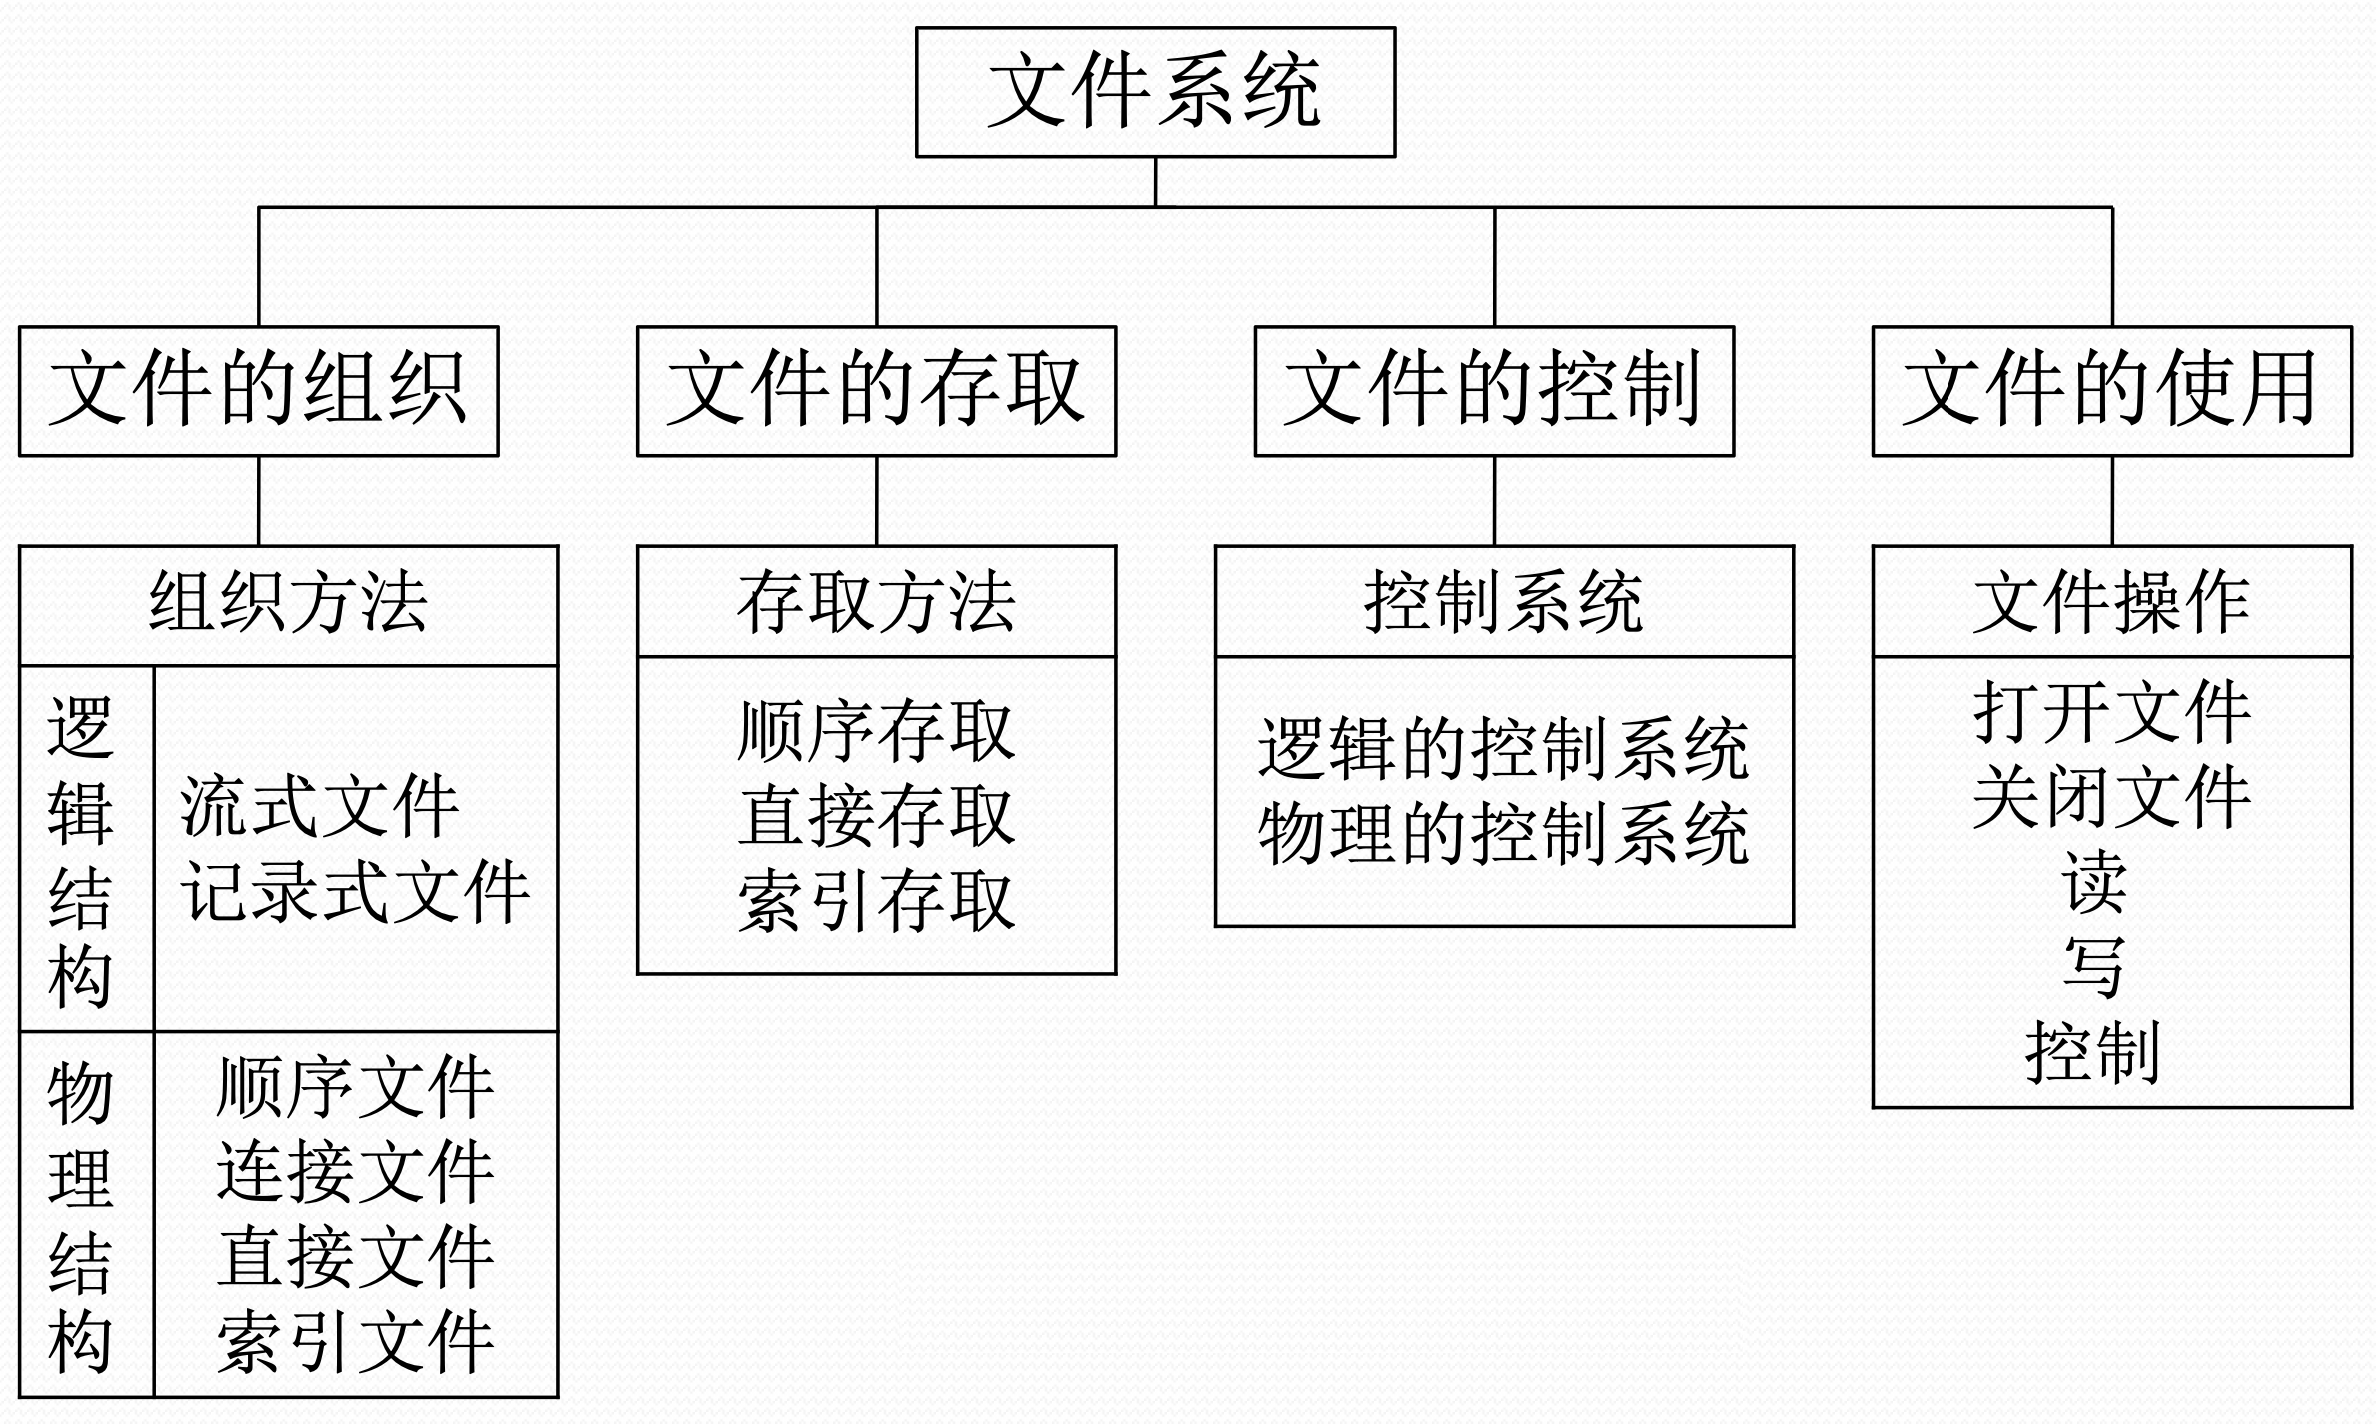
\includegraphics[width=0.65\textwidth]{img/5.1.2.2}
	\end{figure}


	\section{文件的组织}
	\subsection{文件的存储}

	\subsubsection{存储介质}
	常见的文件存储介质有磁带、光盘和磁盘等
	\begin{itemize}
		\item \textbf{卷}是存储介质的物理单位,对应于一盘磁带、一块软盘、一个光盘片或一个硬盘分区
		\item \textbf{块}是存储介质上连续信息所组成的一个区域,也叫做物理记录
		\begin{itemize}
			\item 块是主存储器和辅助存储器进行信息交换的物理单位,每次总是交换一块或整数块信息
		\end{itemize}
	\end{itemize}

	块的大小取决于用户使用方式、数据传输效率和存储设备类型等多种因素
	\begin{itemize}
		\item 不同类型的存储介质,块的长短常常各不相同;对同一类型的存储介质,块的大小一般相同,但也可以不同
		\item 外围设备由于启停机械动作或识别不同块的要求,两个相邻块之间必须留有间隙
		\begin{itemize}
			\item 间隙是块之间不记录用户代码信息的区域
		\end{itemize}
	\end{itemize}


	\subsubsection{存取方法}
	文件存取方法是用户读写文件存储器上的物理记录的方法。操作系统需要为不同类型的存储设备提供不同的存取方法,常用的文件存取方法有顺序存取、直接存取和索引存取
	\begin{itemize}
		\item 顺序存取:严格按照信息的物理位置次序进行定位和读写
		\begin{itemize}
			\item 顺序存取的过程
			\begin{itemize}
				\item 读操作根据读指针读出当前记录,同时推进读指针,指向下一次要读出的记录
				\item 写操作则设置写指针,把一个记录写到文件未端,同时推进写指针
			\end{itemize}
			\item 允许对读指针进行前跳或后退$n$(整数)个记录的操作,即允许对固定长度记录的顺序文件采用随机访问
			\item 顺序存取设备
			\begin{itemize}
				\item 磁带机是最常用的一种顺序存取存储设备,它具有存储容量大、稳定可靠、卷可装卸和便于保存等优点,广泛用作存档
				\item 磁带的一个突出特点是块长的变化范围较大,块可以很小,也可以很大,原则上没有限制
				\item 光盘也是一种顺序存取存储设备,光盘上的磁道不是同心圆,而是螺旋形的,本质上也是线性的
			\end{itemize}
		\end{itemize}
		\item 直接存取:可以非顺序地从文件中的任何位置存取文件内容,也叫随机存取
		\begin{itemize}
			\item 很多应用场合要求快速地以任意次序直接读写某个记录。例如对于航空订票系统,用航班号作标识,把特定航班的所有信息存放在物理块中,用户预订某航班时,直接计算出该航班的存位置
			\item 直接存取设备,也叫随机存取存储设备。以下以磁盘为例进行说明
			\begin{itemize}
				\item 通过移臂与旋转两维寻址,存取速度高
				\item 它的每个物理记录有确定的位置和唯一的地址,存取任何一个物理块所需的时间几乎不依赖于此信息的位置
			\end{itemize}
		\end{itemize}
		\item 索引存取:基于索引文件的索引存取方法
		\begin{itemize}
			\item 文件的记录不按位置而是按其记录名和记录键来编址,所以用户提供记录名或记录键之后,先按名查找,再查找需要的记录
			\begin{itemize}
				\item 采用记录键时,往往按照一种次序如字母序进行顺序存放
				\item 除可采用按键存取外,也可以采用顺序存取或直接存取的方法
			\end{itemize}
			\item 在实际的系统中,大都采用多级索引,以加速记录查找过程
		\end{itemize}
	\end{itemize}

	\subsection{文件的逻辑结构}

	\subsubsection{逻辑文件}
	\textbf{逻辑文件},又称为\textbf{文件的逻辑结构}
	\begin{itemize}
		\item 是独立于物理环境的用户概念中的抽象信息组织方式
		\item 也是用户能观察到并加以处理的数据集合
		\item 文件的逻辑结构分为两种形式
		\begin{itemize}
			\item 基于字节的\textbf{流式文件}
			\item 基于记录的\textbf{记录式文件}
		\end{itemize}
	\end{itemize}

	\subsubsection{流式文件}
	流式文件是\textbf{无结构}文件,是指文件内的数据不再组成记录,只是由一串依次的字节组成的信息流序列,即字节流文件
	\begin{itemize}
		\item 这种文件常常按长度来读取所需信息,也可以用插入的特殊字符作为分界
		\item 全部文件存储都可以抽象为流式文件,因而大多数操作系统只提供流式文件
	\end{itemize}
	
	\subsubsection{记录式文件}
	记录式文件是一种有结构的文件,它是若干逻辑记录信息所组成的记录流文件
	\begin{itemize}
		\item 逻辑记录是文件中按信息在逻辑上的独立含义所划分的信息单位
		\item 例如对于下图而言,每个职工的工资信息是一个逻辑记录,整个单位职工的工资信息便组成了该单位工资信息的记录式文件
	\end{itemize}
	\begin{figure}[H]
		\centering
		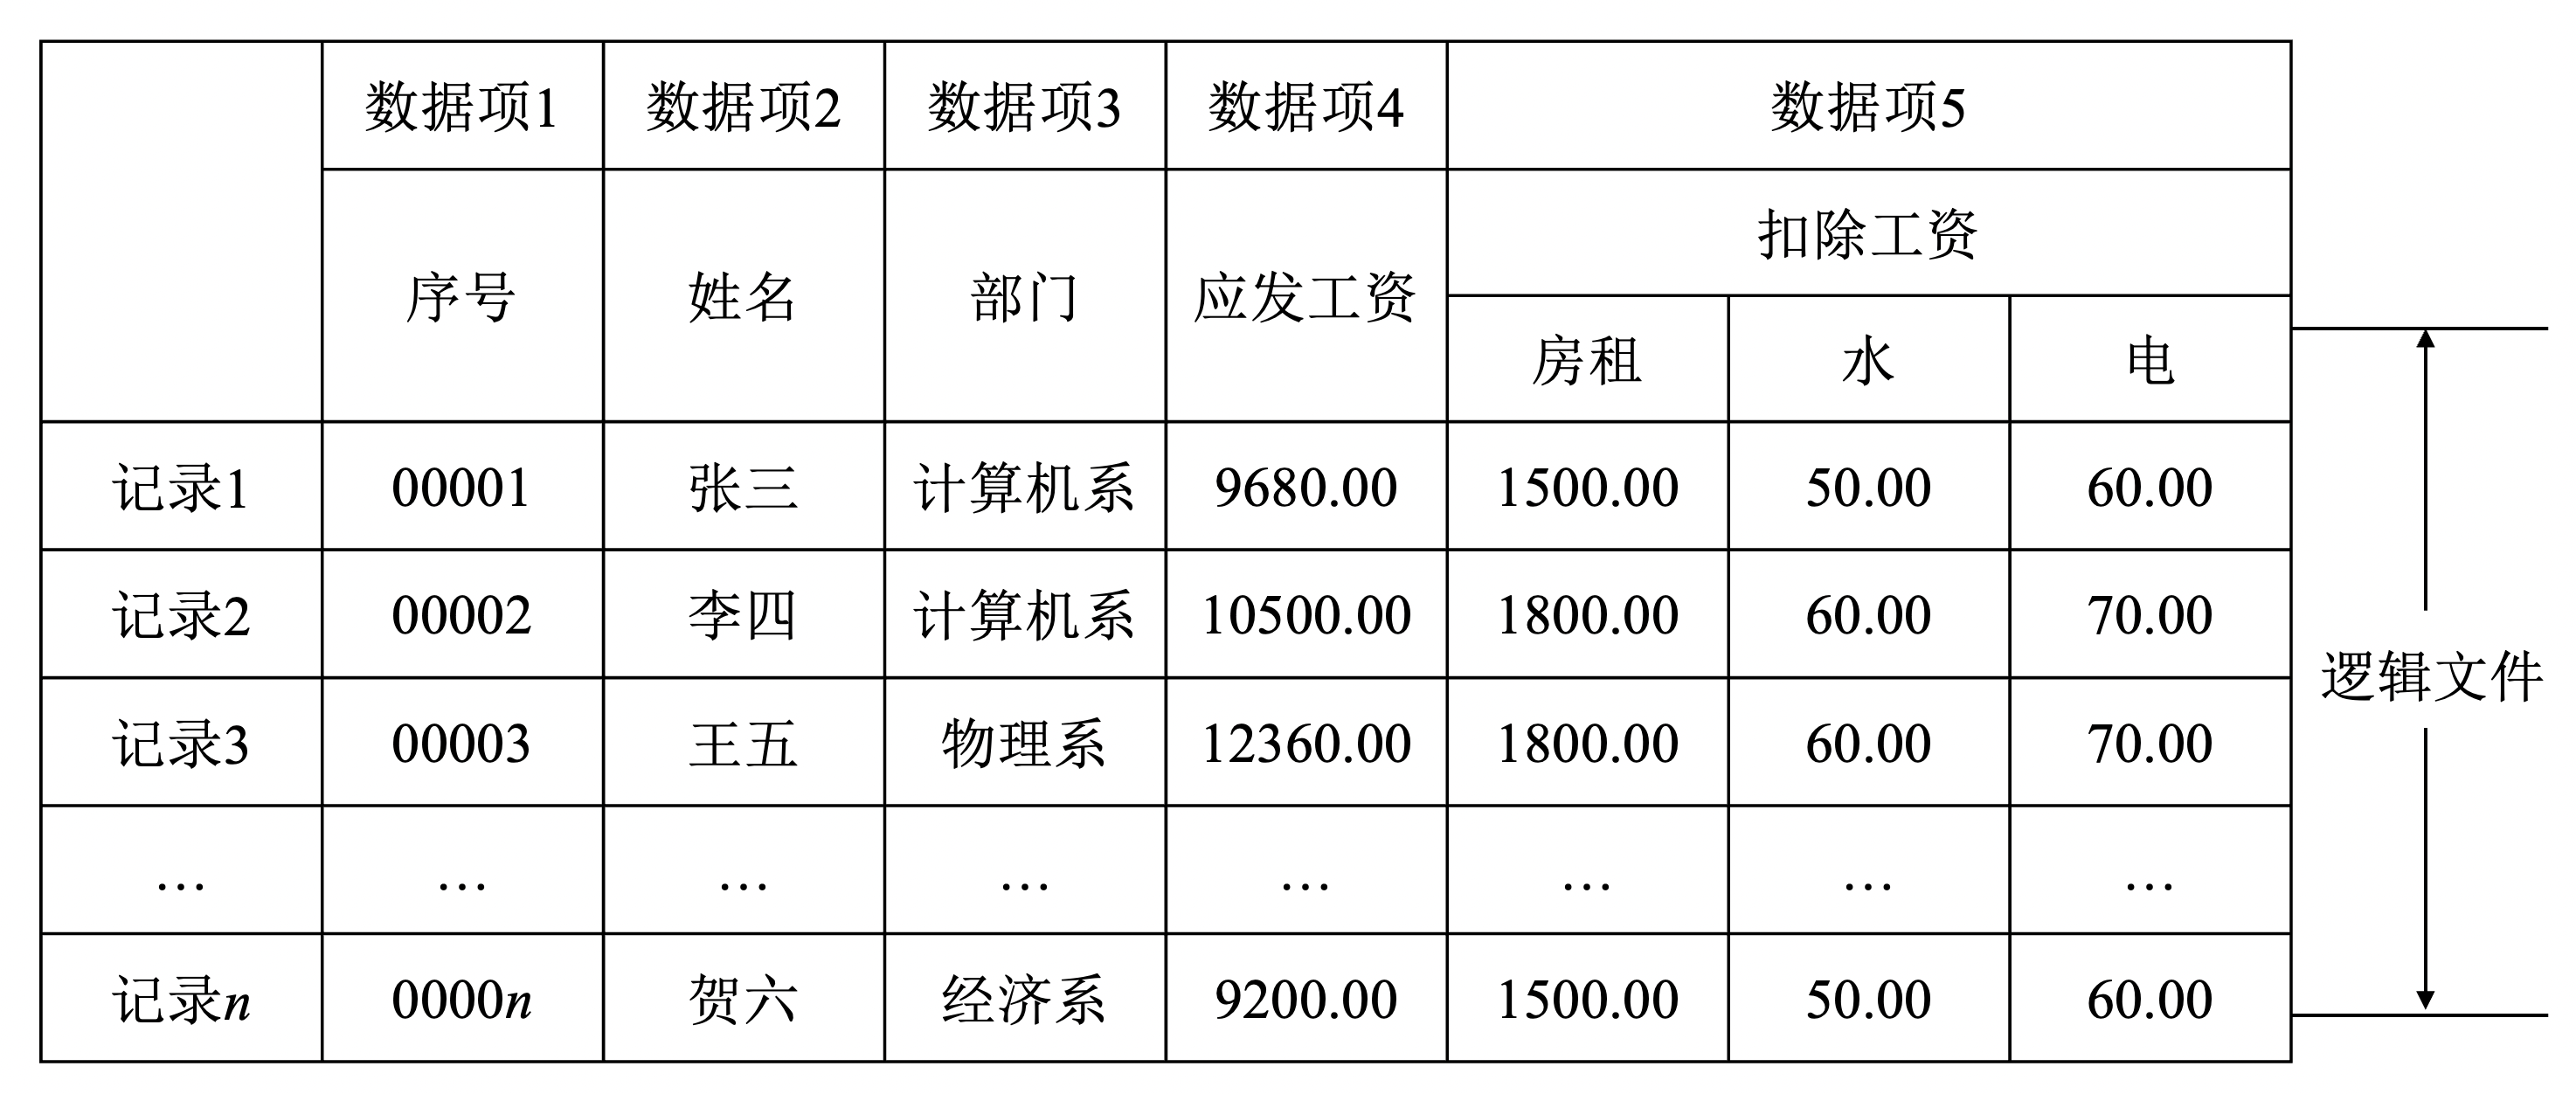
\includegraphics[width=0.7\textwidth]{img/5.2.2.3}
	\end{figure}

	记录式文件与数据库
	\begin{itemize}
		\item 数据库管理系统也支持逻辑记录
		\item 但数据库有别于记录式文件,数据库中的记录之间可以通过数据冗余构成某种联系
		\item 数据库管理系统支持基于联系的数据查询,文件系统则不支持
	\end{itemize}

	\subsection{记录的成组与分解}

	\subsubsection{记录成组与分解的提出}
	在大多数情况下,一个逻辑记录的大小远远小于物理记录,若一个物理记录只存放一个逻辑记录就会造成存储空间的浪费,并且导致重复启动外围设备,降低计算机处理效率
	\begin{itemize}
		\item 为了解决这一问题,可以将若干个逻辑记录合并成一组,写入一个块中,这种处理方式称为\textbf{记录的成组},每个物理块中逻辑记录的个数称为\textbf{块因子}
		\item 对于流式文件,一个物理记录可以存放很多个连续字节
	\end{itemize}

	\subsubsection{记录成组与分解操作}
	系统设置独立于用户数据区的输入/输出缓冲区
	\begin{itemize}
		\item 记录的成组操作:在输出缓冲区内进行,凑满一块后才将缓冲区内的信息写到存储介质上
		\item 记录的分解操作:当存储介质上的一个物理记录读进输入缓冲区后,把逻辑记录从块中分离出来
	\end{itemize}
	\begin{figure}[H]
		\centering
		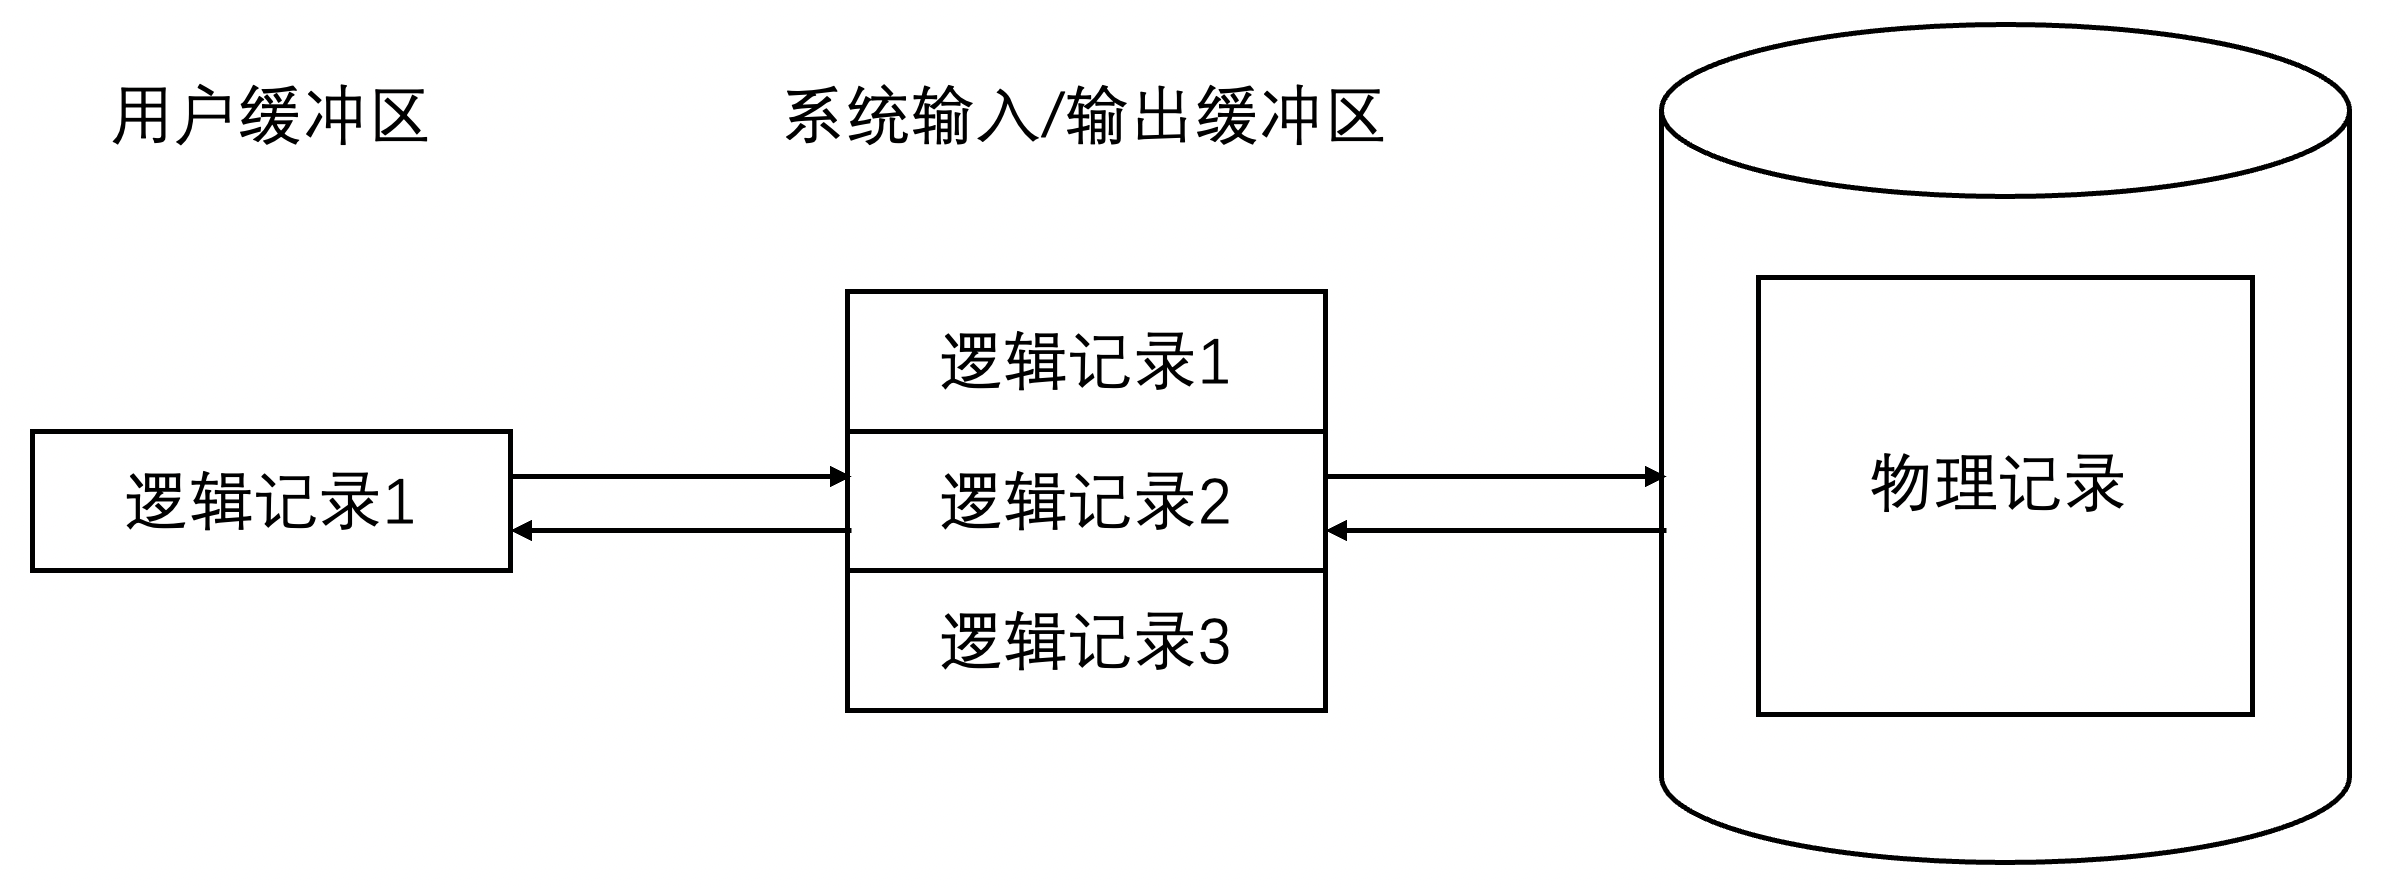
\includegraphics[width=0.6\textwidth]{img/5.2.3.2}
	\end{figure}

	\subsubsection{记录成组与分解的特征}
	\begin{itemize}
		\item 记录成组与分解的优点:不仅节省存储空间,还能减少输入输出操作次数,提高系统效率
		\item 记录成组与分解处理带来的新特征:
		\begin{itemize}
			\item 提前读:用户的读请求会导致包含该逻辑记录的物理块读入输入缓冲区,这一操作可能读入了多个逻辑记录,可以更快的访问附近的记录
			\item 推迟写:对于用户的写请求,逻辑记录首先写入输出缓冲区,只有当该缓冲区中的逻辑记录满后才会引起实际的输出
		\end{itemize}
		\item 记录成组与分解的副作用:因为数据优先写到输出缓冲区,等到缓冲区满才会写到磁盘,可能会造成数据不一致
	\end{itemize}

	\subsection{文件的物理结构}
	文件的物理结构和组织是指逻辑文件在物理存储空间中的存放方法和组织关系,又称物理文件
	\begin{itemize}
		\item 文件的存储结构涉及块的划分、记录的排列、索引的组织、信息的搜索等许多问题
		\item 文件存储结构的优劣直接影响文件系统的性能
	\end{itemize}

	\subsubsection{顺序文件}
	顺序文件:将一个文件中逻辑上连续的信息存放到存储介质的依次相邻的块中形成顺序结构,又称连续文件
	\begin{itemize}
		\item 磁带文件、光盘文件是典型例子且批处理文件,系统文件用得最多
		\item 顺序文件的特点
		\begin{itemize}
			\item 优点:顺序存取记录时速度较快
			\item 缺点:建立文件前需要能预先确定文件长度,以便分配存储空间;修改、插入和增加文件记录有困难
		\end{itemize}
	\end{itemize}

	\subsubsection{连接文件}
	连接文件:使用连接字(指针)来表示文件中各条记录之间的关系
	\begin{itemize}
		\item 又称串联文件,输入井、输出井都是此类文件
		\item 第一块文件信息的物理地址由文件目录给出,而每一块的连接字指出了文件的下一个物理块位置;连接字内容为0时,表示文件至本块结束
		\item 连接文件的特点
		\begin{itemize}
			\item 优点:易于对文件记录做增、删、改,易于动态增长记录;不必预先确知文件长度;存储空间利用率高
			\item 缺点:存放指针需额外的存储空间;由于存取须通过缓冲区,待获得连接字后,才能找到下一物理块的地址,因而仅适用于顺序存取
		\end{itemize}
	\end{itemize}

	\begin{figure}[H]
		\centering
		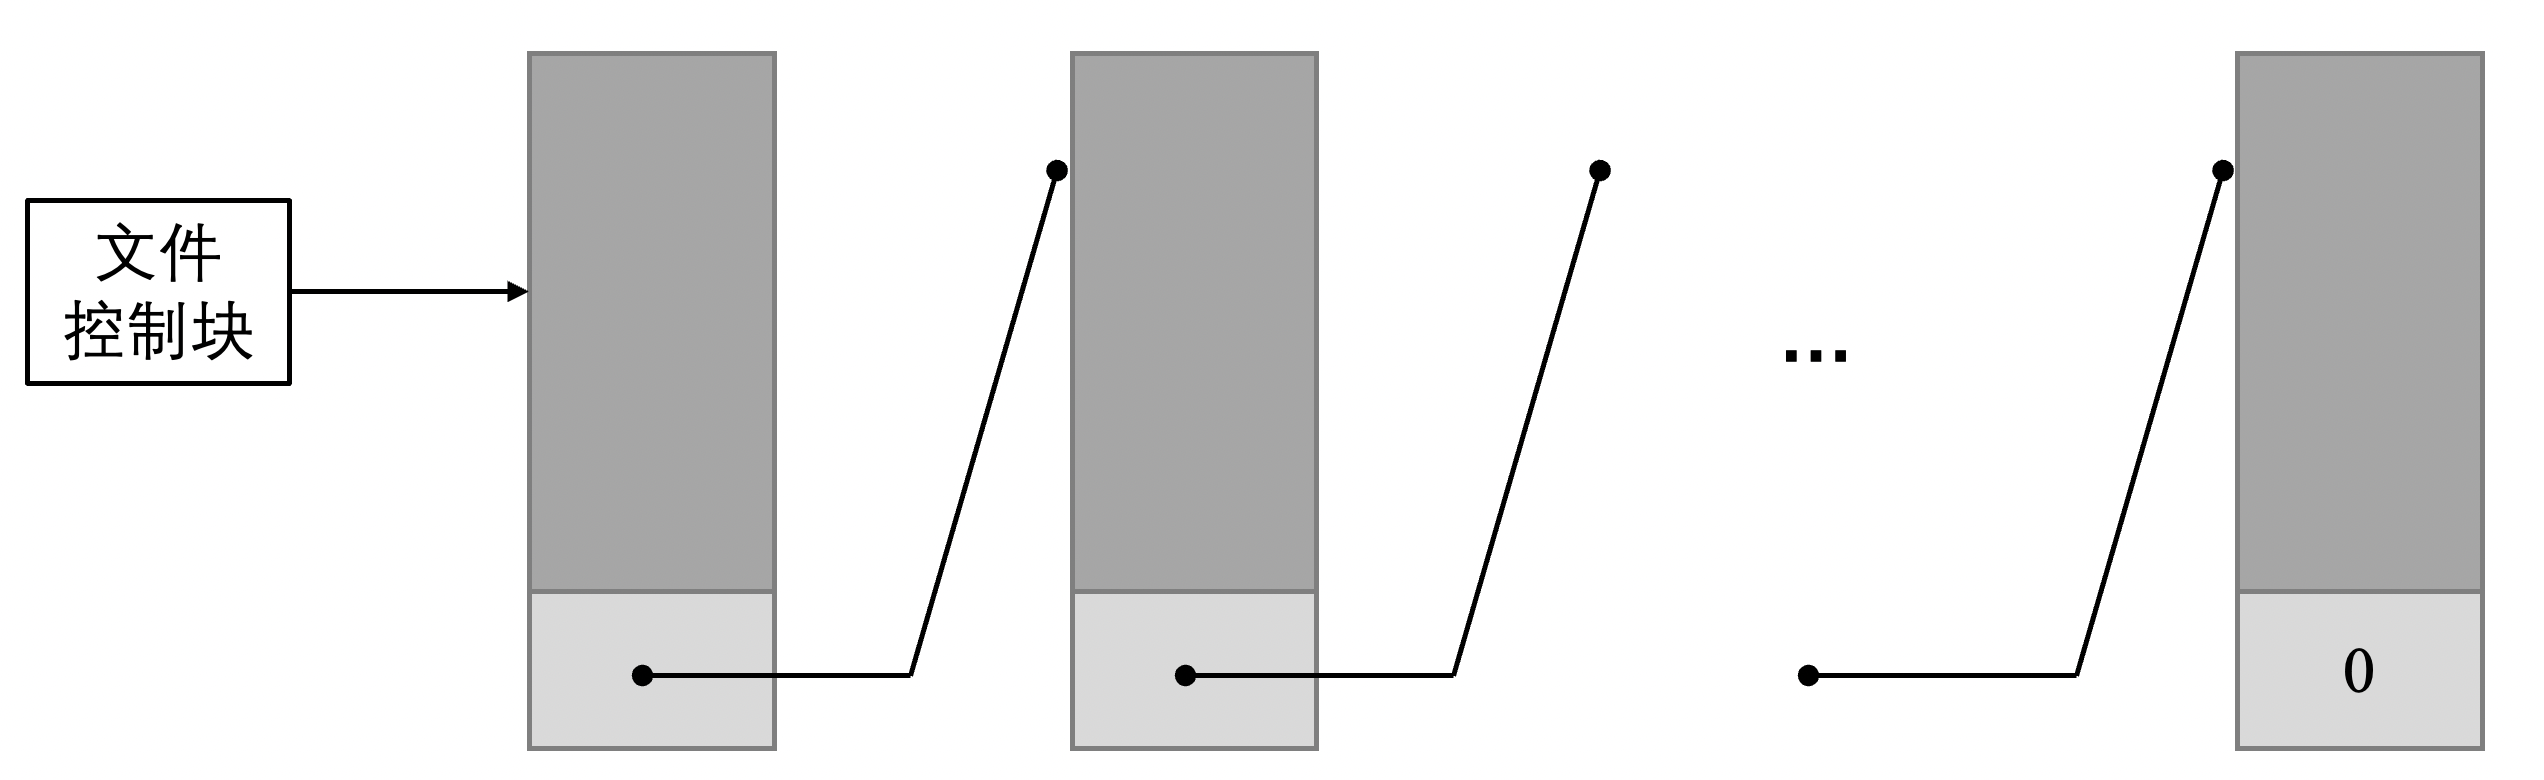
\includegraphics[width=0.65\textwidth]{img/5.2.4.2}
	\end{figure}


	\subsubsection{直接文件}
	直接文件:通过计算记录的关键字建立与其物理存储地址之间的对应关系,又称散列文件
	\begin{itemize}
		\item 这种变换通常采用散列法(hash法)
		\item 计算寻址结构可能出现冲突,即不同的关键字可能变换出相同的地址来,解决办法有拉链法、循环探查法、二次散列法、溢出区法等
	\end{itemize}

	\subsubsection{索引文件}
	索引文件:为每个文件建立了一张索引表,其中每个表目包含一个记录的键(或逻辑记录号)及其存储地址
	\begin{itemize}
		\item 索引表的地址可由文件目录指出,查阅索引表先找到相应记录键(或逻辑记录号),然后获得数据存储地址
	\end{itemize}
	\begin{figure}[H]
		\centering
		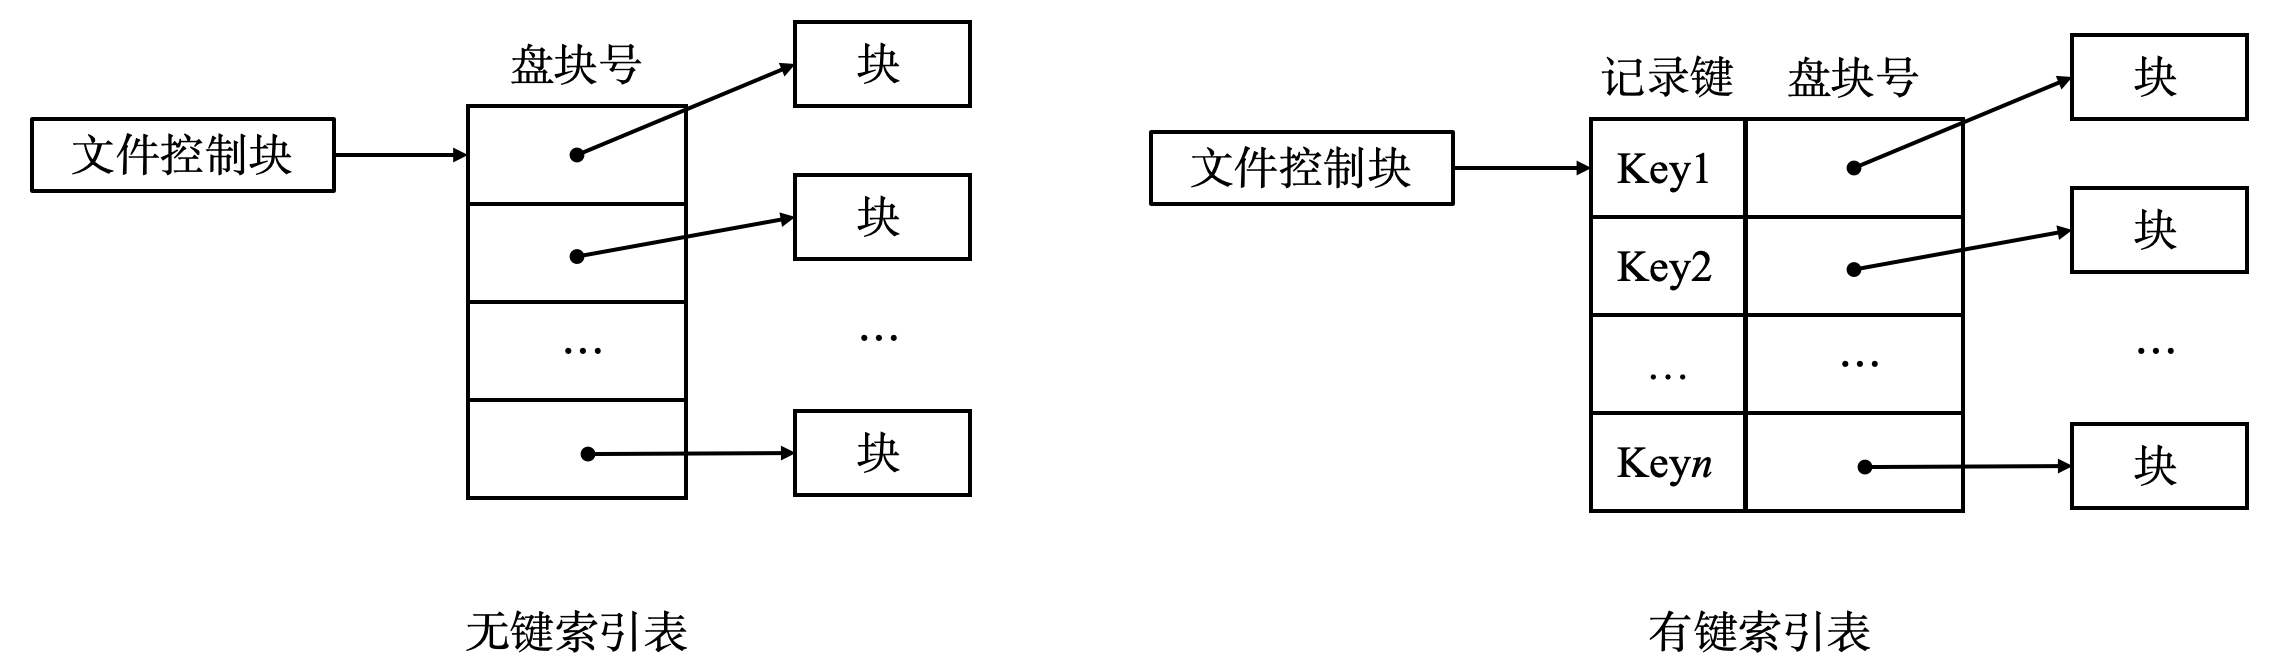
\includegraphics[width=0.8\textwidth]{img/5.2.4.4.1}
	\end{figure}

	索引文件的访问方式
	\begin{itemize}
		\item 索引文件在文件存储器上分为两个区:索引区和数据区
		\item 访问索引文件需两步操作:第一步查找索引表,第二步获得记录物理地址
		\item 需要两次访问辅助存储器,若文件索引已预先调入主存储器,那么就可减少一次内外存信息交换
	\end{itemize}

	索引文件的特点
	\begin{itemize}
		\item 索引结构可以被认为是连接结构的一种扩展,除了具备连接文件的优点外,还克服了它只能作顺序存取的缺点,具有直接读写任意一个记录的能力,便于文件的增、删、改
		\item 索引文件的缺点是:增加了索引表的空间开销和查找时间
	\end{itemize}

	索引表的组织有一级索引、二级索引和多重索引等组织结构。下图为Unix操作系统采用的多重索引结构
	\begin{figure}[H]
		\centering
		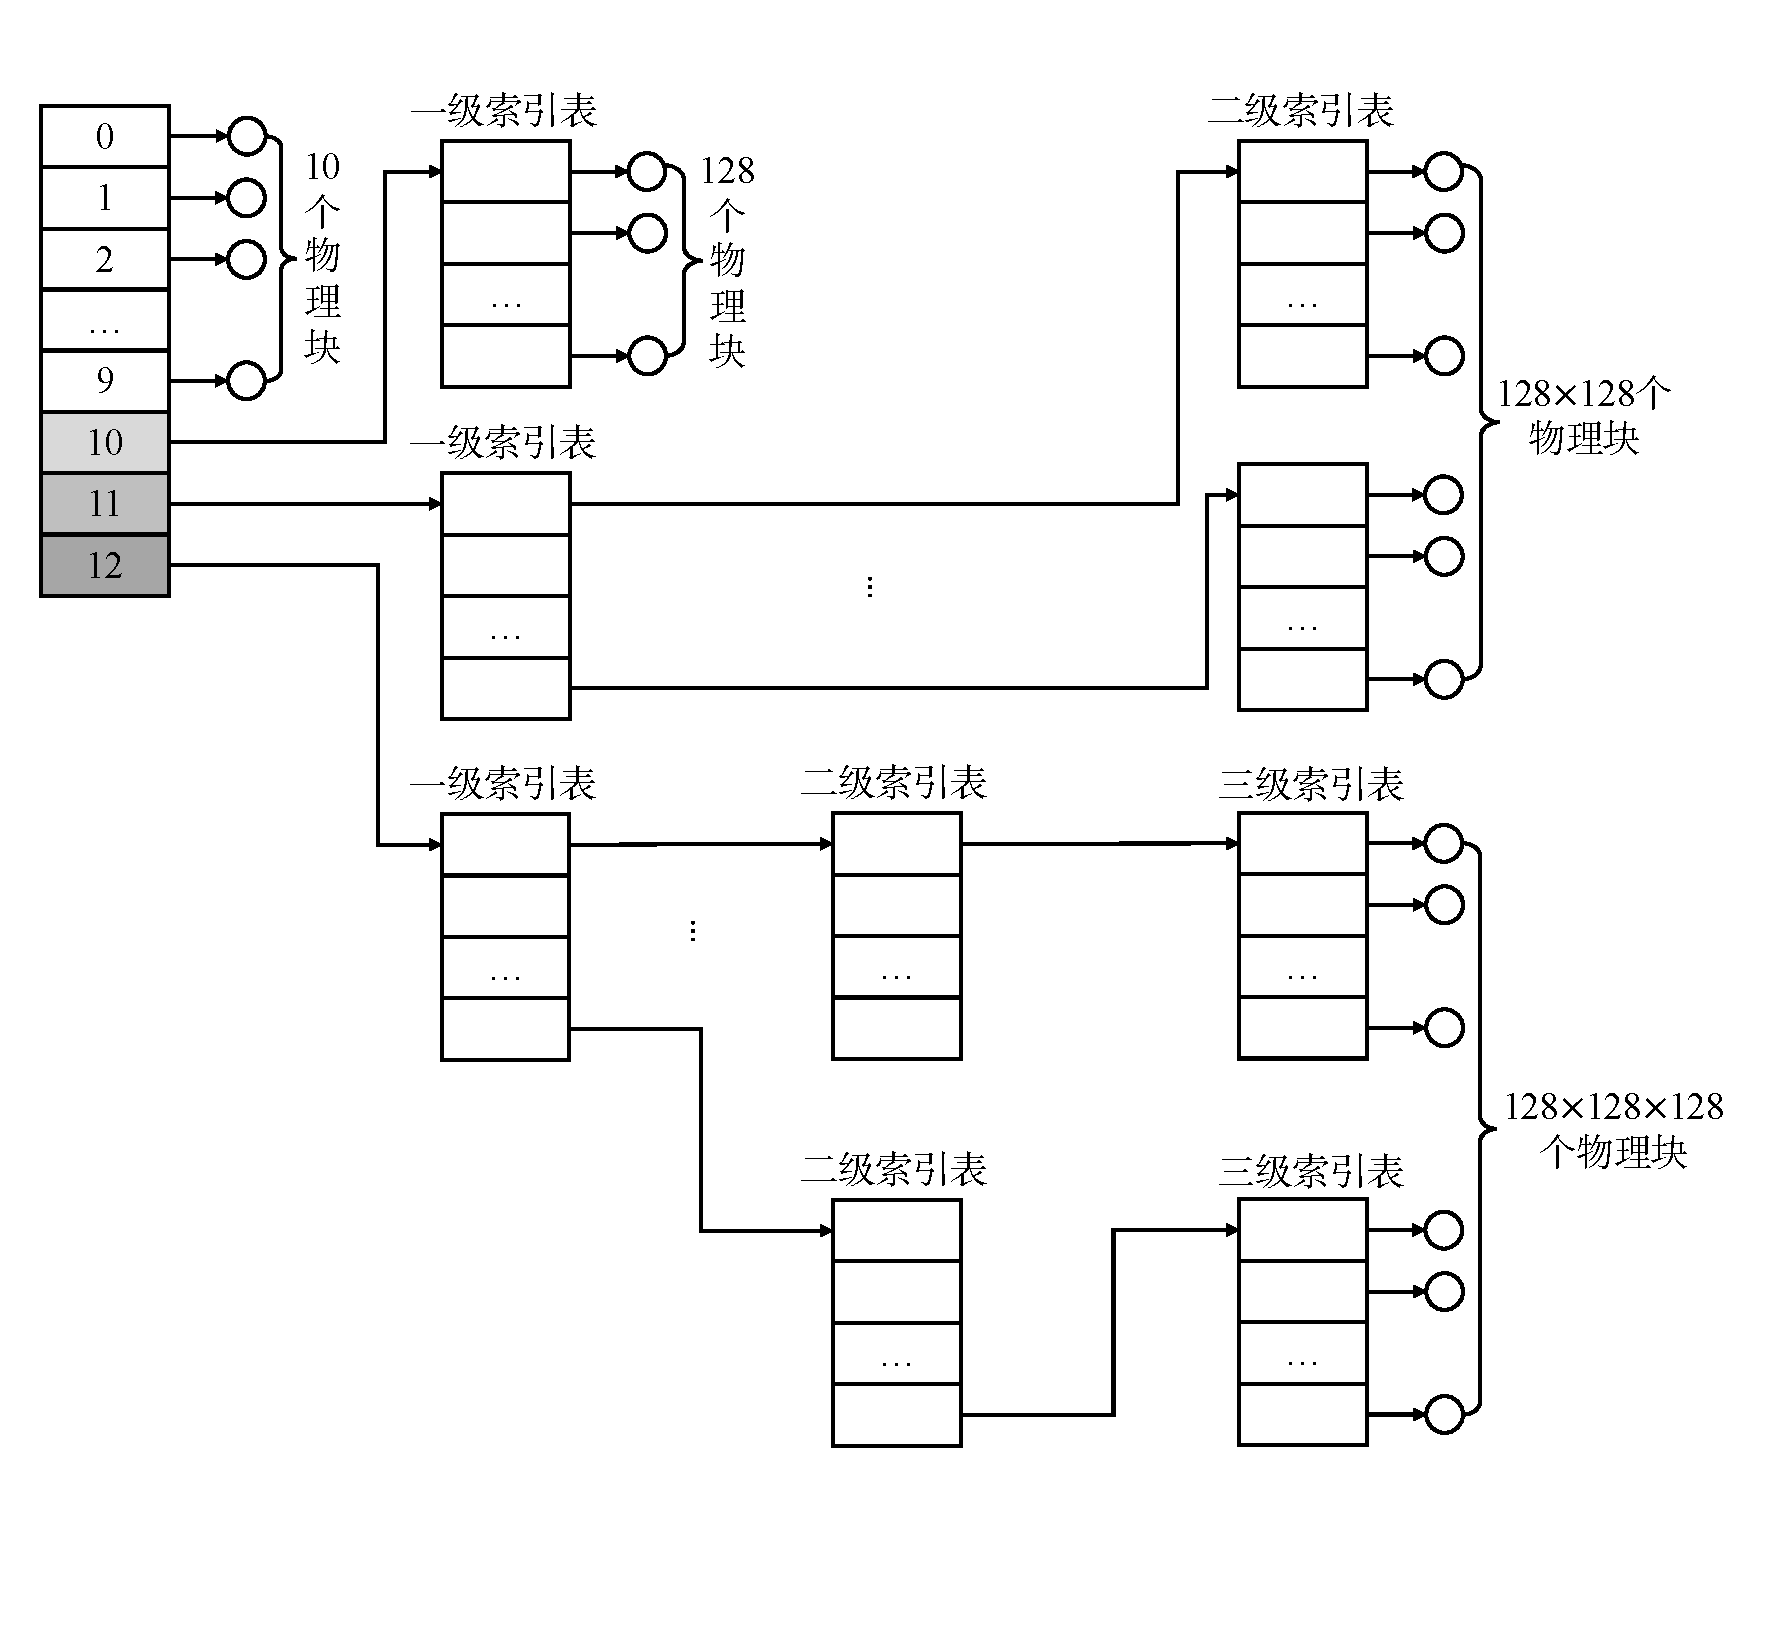
\includegraphics[width=0.85\textwidth]{img/5.2.4.4.2}
	\end{figure}

	\begin{itemize}
		\item 系统仅提供流式文件,每个文件的索引表规定为13个索引项
		\item 前10项(0 $\sim$ 9项)登记一个存放文件信息的物理块号,称为直接寻址
		\item 如果文件大于10块,则利用第11项(序号10)指向一个物理块,该块中最多可以放128个存放文件信息的物理块号,称为一次间接寻址
		\item 进而还可以利用第12项(序号11)和第13项(序号12)做第二次和三次间接寻址
	\end{itemize}

	\textbf{例:}在UNIX系统中,每个$i$节点中分别含有10个直接地址的索引和一、二、三级间接索引。若每个盘块放128个盘块地址,则一个1MB的文件分别占用多少各级索引所使用的数据物理块?20MB的文件呢?假设每个盘块有512B。

	\begin{center}
		\begin{tcolorbox}[colback=white,%gray background
			colframe=black,% black frame colour
			width=\textwidth,
			arc=1mm, auto outer arc,
			boxrule=0.75pt,
		   ]
		直接块容量$=10\times 512\mathrm{B}/1024=5\mathrm{KB}$ 
		
		一次间接块容量$128\times 512\mathrm{B}/1024=64\mathrm{KB}$

		二次间接块容量$=128\times 128\times 512\mathrm{B}/1024=8192\mathrm{KB}$

		三次间接块容量$=128\times 128\times 128\times 512\mathrm{B}/1024=1048576\mathrm{KB}$

		对于1MB的文件而言,占满直接块和一次间接块,还需要$1024\mathrm{KB}-5\mathrm{KB}-64\mathrm{KB}=955\mathrm{KB}$的二次间接块,即$955\times 1024\mathrm{B}/512\mathrm{B}=1910$块。所以1MB的文件分别占用1910个二次间接盘块,128个一次间接盘块。

		对于20MB的文件而言,占满直接块、一次间接块和二次间接块,还需要$20\times 1024\mathrm{KB}-5\mathrm{KB}-64\mathrm{KB}-8192\mathrm{KB}=12219\mathrm{KB}$的三次间接块,即$12219\times 1024\mathrm{B}/512\mathrm{B}=24438$块。所以20MB的文件分别占用24438个三次间接盘块,$128\times 128=16384$个二次间接盘块和128个一次间接盘块。
		\end{tcolorbox}
	\end{center}

	\section{文件系统调用的实现}
	文件系统提供给用户程序的一组系统调用,包括:创建、删 除、打开、关闭、读、写和控制,通过这些系统调用用户能获得文件系统的各种服务
	
	\subsection{文件系统的结构}

	\subsubsection{磁盘扇区序列划分}
	\begin{itemize}
		\item 引导块:占用0\#号块
		\begin{itemize}
			\item 位于文件卷最开始的第一扇区,是文件系统的引导代码
		\end{itemize}
		\item 超级块:占用1\#号块
		\begin{itemize}
			\item 存放文件系统结构和管理信息
			\begin{itemize}
				\item 例如记录inode表所占盘块数
				\item 文件数据所占盘块数
				\item 主存中登记的空闲盘块数
				\item 主存中登记的空闲块物理块号
				\item 主存中登记的空闲inode数
				\item 主存中登记的空闲inode编号
				\item 以及其他文件管理控制信息
			\end{itemize}
			\item 可见超级块既有盘位示图的功能,又记录整个文件卷的控制数据
			\item 每当一个块设备作为文件卷被安装时,该设备的超级块就要复制到主存系统区中备用,而拆卸文件卷时,修改过的超级块需复制回磁盘的超级块中
		\end{itemize}
		\item 索引节点区:占用$2\# \sim (k+1)\#$块
		\begin{itemize}
			\item 存放inode表:每个文件都有各种属性,它们被记录在称为索引节点inode的结构中
			\begin{itemize}
				\item 所有inode都有相同的大小,且inode表是inode结构的列表,文件系统中的每个文件在该表中都有一个inode
			\end{itemize}
			\item 分为磁盘inode表和主存活动inode表,后者可以解决频繁访问磁盘inode表的效率问题
		\end{itemize}
		\item 数据区:占用 $(k+2)\# \sim n\#$块
		\begin{itemize}
			\item 文件的内容保存在这个区域,磁盘上所有物理块的大小是一样的,如果文件包含超过一块的数据,则文件内容会存放在多个盘块中
		\end{itemize}
	\end{itemize}

	\begin{figure}[H]
		\centering
		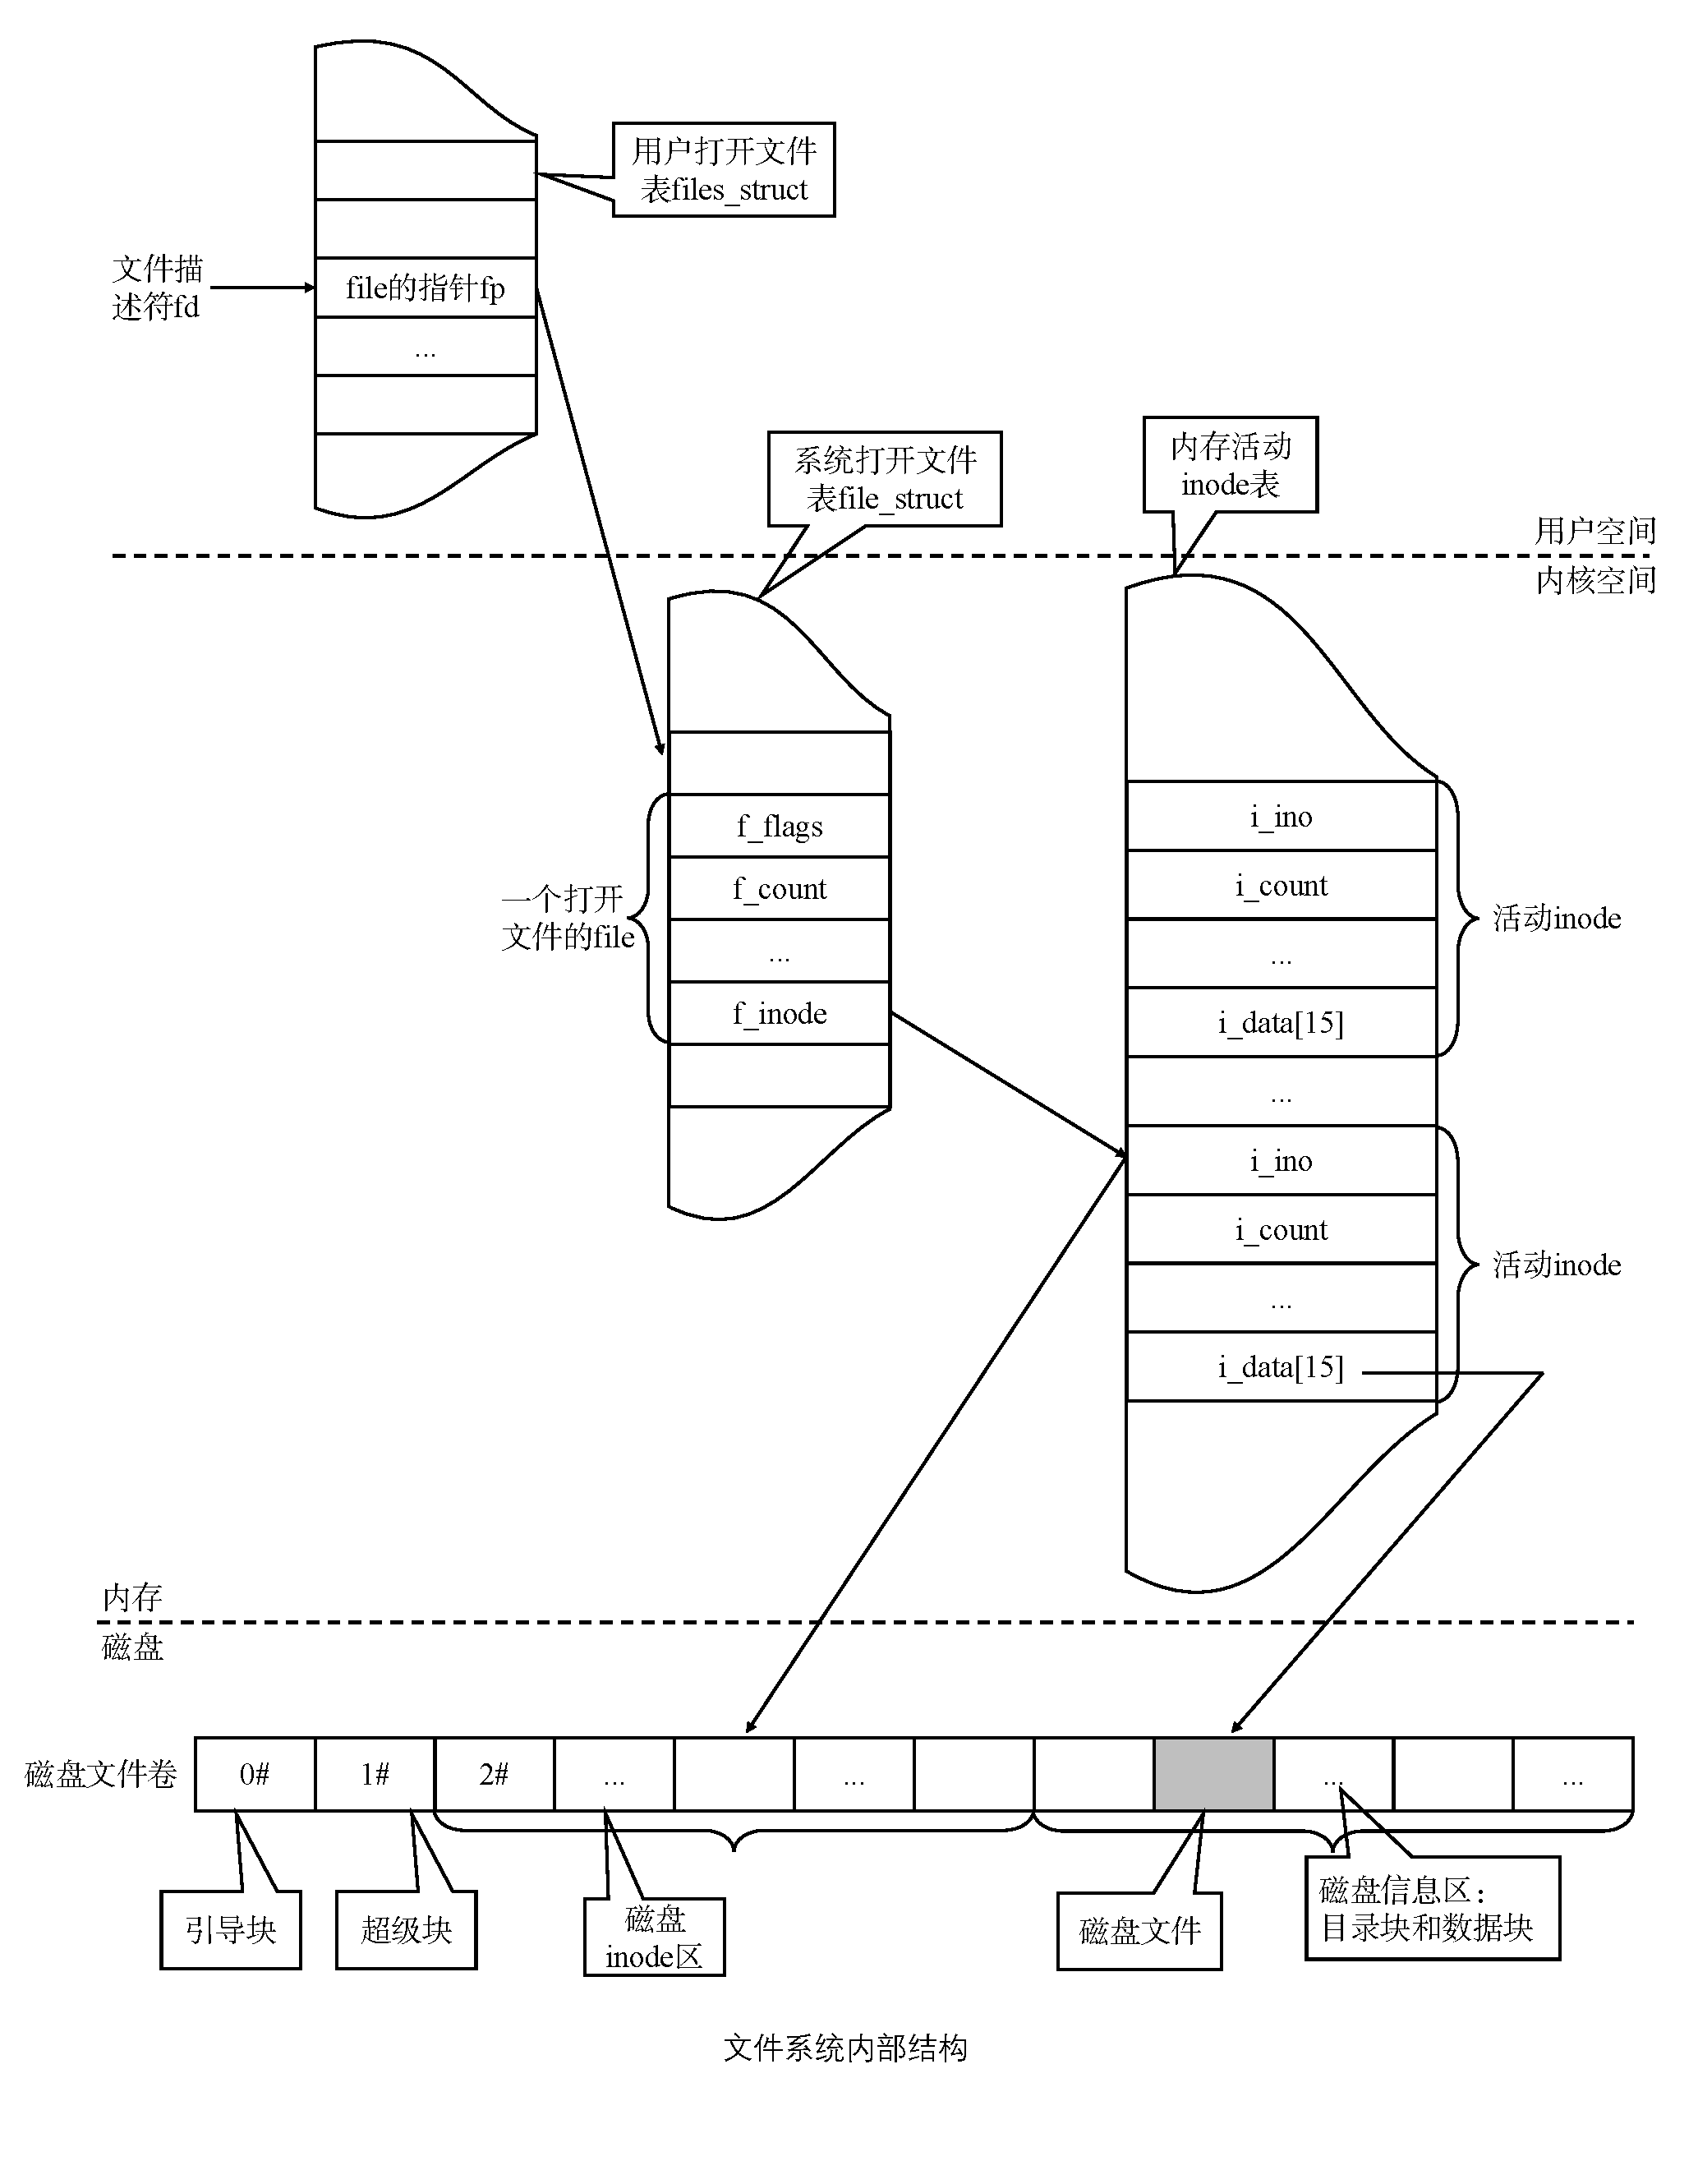
\includegraphics[width=0.95\textwidth]{img/文件系统内部结构.pdf}
	\end{figure}

	\subsubsection{内存中重要的数据结构}

	\begin{itemize}
		\item 用户打开文件表:进程的PCB结构中保留一个\ \verb|files_struct|,称为用户打开文件表或文件描述符表
		\begin{itemize}
			\item 表项的序号为文件描述符fd
			\item 该登记项内登记系统打开文件表的一个入口指针fp
			\item 通过此系统打开文件表项连接到打开文件的活动inode
		\end{itemize}
		\item 系统打开文件表:为解决多用户进程共享文件、父子进程共享文件设置的系统数据结构\ \verb|file_struct|
		\begin{itemize}
			\item 主存专门开辟最多可登记256项的系统打开文件表区,当打开一个文件时,通过此表项把用户打开文件表的表项与文件活动inode联接起来,以实现数据的访问和信息的共享
		\end{itemize}
		\item 主存活动inode表:为解决频繁访问磁盘索引节点inode表的效率问题,系统开辟的主存区
		\begin{itemize}
			\item 正在使用的文件的inode被调入主存活动索引节点inode中,以加快文件访问速度
		\end{itemize}
	\end{itemize}

	\begin{figure}[H]
		\centering
		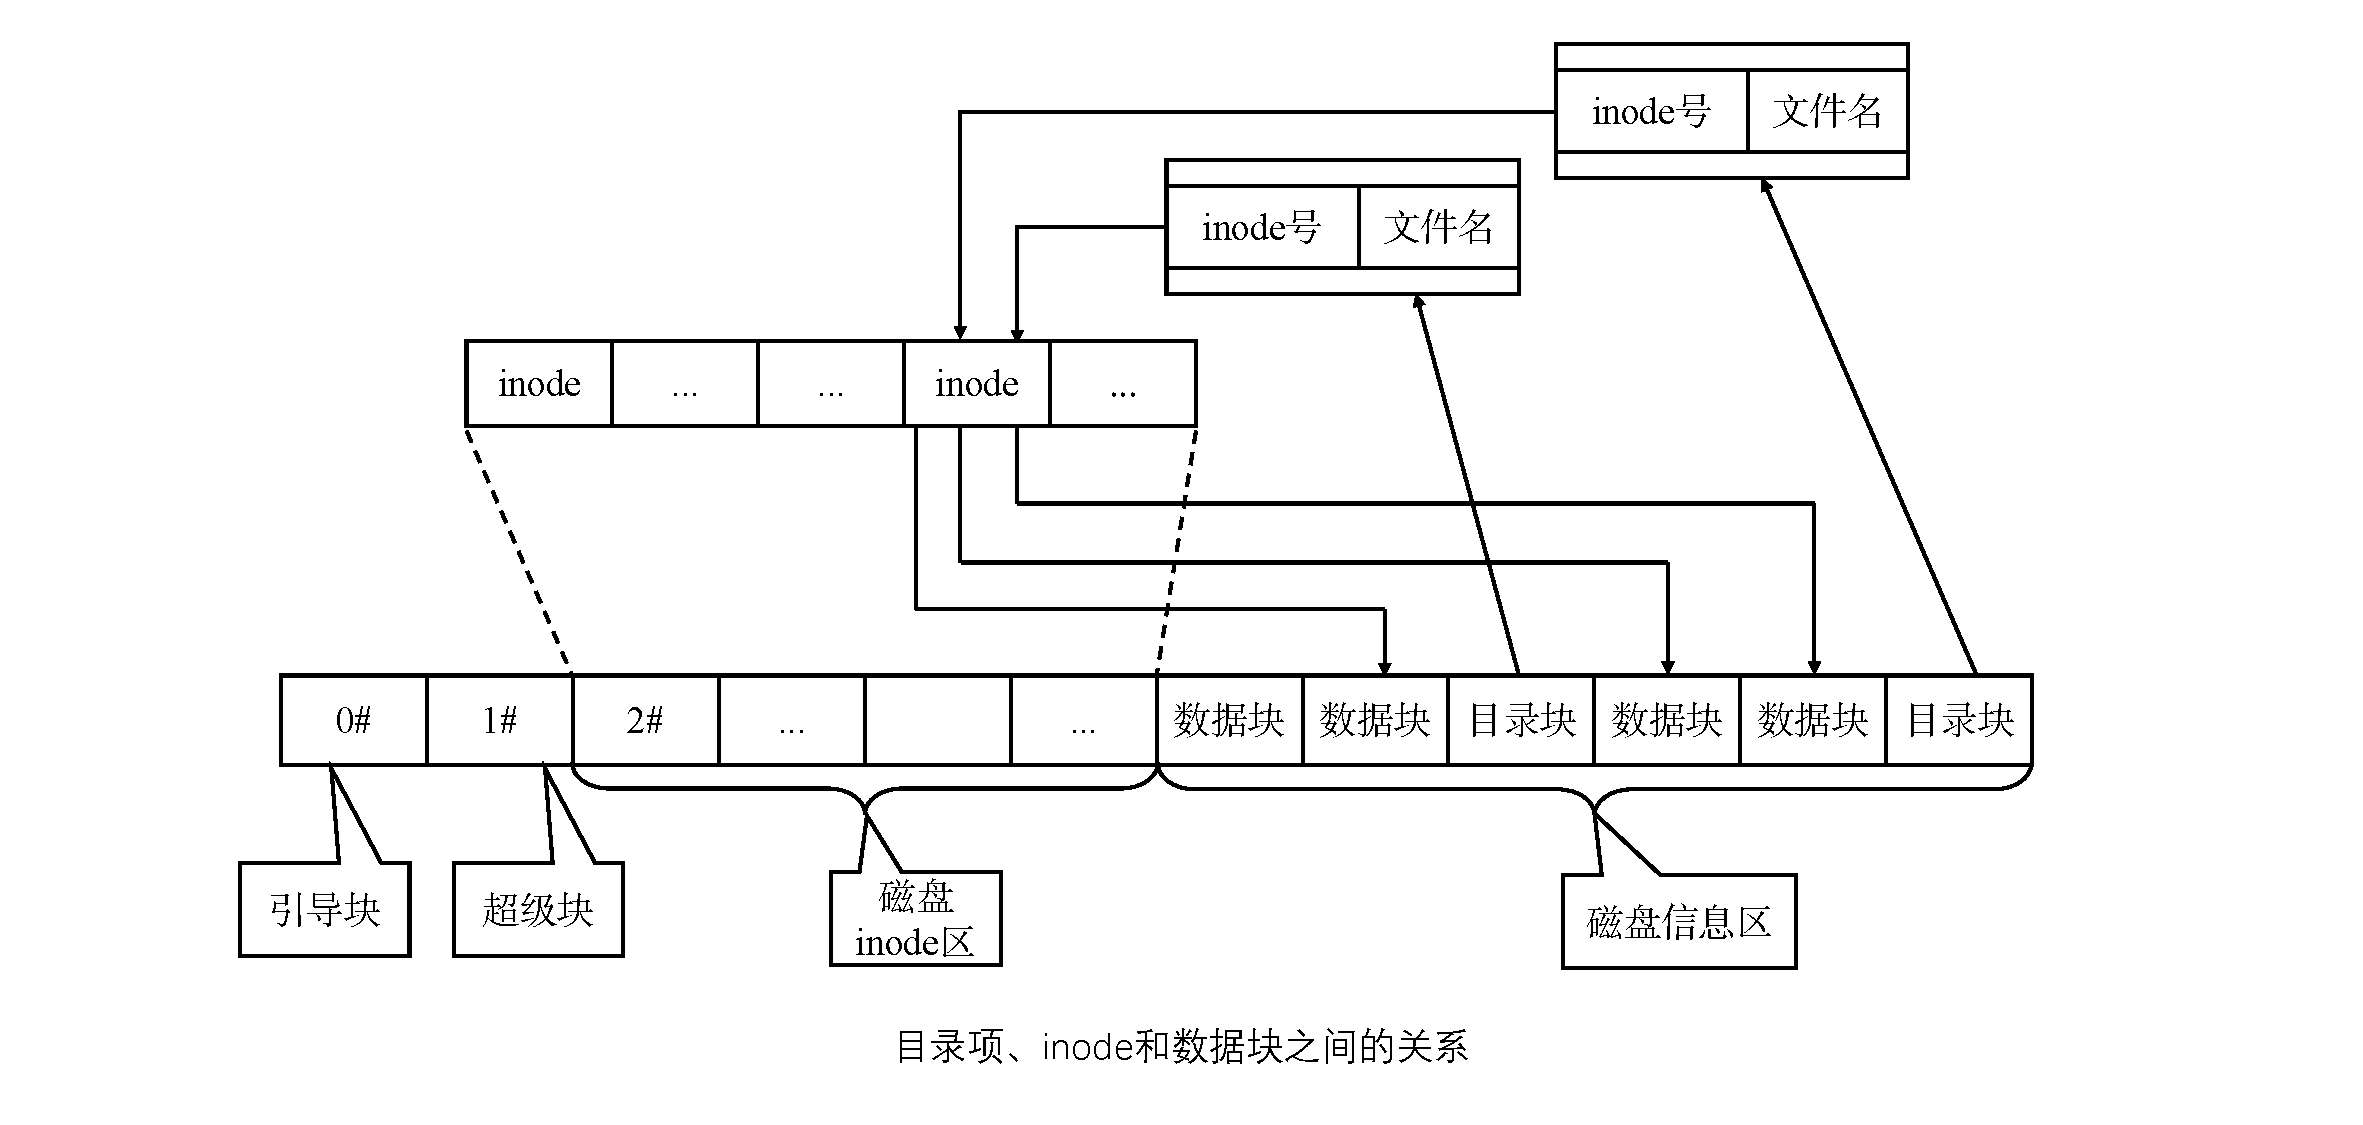
\includegraphics[width=0.95\textwidth]{img/目录项、inode和数据块之间的关系.pdf}
	\end{figure}

	\subsection{文件系统调用}
	用户通过两类接口与文件系统联系,通过这些系统调用,用户能够获得文件系统的各种服务
	\begin{itemize}
		\item 第一类是与文件有关的操作命令,例如UNIX中的cat,cd,cp,find,mv,rm,mkdir,rmdir等
		\item 第二类是提供给用户程序使用的文件类系统调用,基本文件类系统调用有:建立、撤销、打开、关闭、读/写、定位
	\end{itemize}

	\subsubsection{文件的创建}
	\begin{lstlisting}[language=C,keywordstyle=\color{black}]
int fd;           // 创建成功后系统返回的文件描述符
int mode;         // 文件所具有的权限
char *filenamep;  // 指向要创建的文件路径名的字符串指针
fd = create(filenamep, mode);		
	\end{lstlisting}

	文件创建的执行过程
	\begin{enumerate}[label=\arabic*.]
		\item 为新文件分配索引节点和活动索引节点,并把索引节点编号与文件分量名组成新目录项,记到目录中
		\item 在新文件所对应的活动索引节点中置初值,如置存取权限i\_mode,连接计数i\_nlink等
		\item 分配用户打开文件表项和系统打开文件表项,置表项初值,读写位移f\_offset清0
		\item 把各表项及文件对应的活动索引节点用指针连接起来,把文件描述字返回给调用者
	\end{enumerate}

	\subsubsection{文件的撤销}
	当不再需要使用一个文件时,可执行撤销文件的操作,又称删除文件
	\begin{itemize}
		\item 在执行删除时,必须要求用户对该文件具有“写”操作权
		\item 删除文件的处理流程:若文件没有关闭,先关闭文件;若为共享文件,则需进行相应的联访处理,然后在目录文件中删去相应目录项,最后释放文件占用的文件存储空间
	\end{itemize}

	\subsubsection{文件的打开}
	\begin{lstlisting}[language=C,keywordstyle=\color{black}]
int fd, mode;
char * filenamep;
fd = open(filenamep, mode);		
	\end{lstlisting}

	打开文件用于建立文件和用户进程之间的使用联系
	\begin{enumerate}[label=\arabic*.]
		\item 检索目录,把它的外存索引节点复制到活动索引节点表
		\item 根据参数mode核对权限,如果非法,则这次打开失败
		\item 当“打开”合法时,为文件分配用户打开文件表项和系统打开文件表项,并为表项设置初值
		\begin{itemize}
			\item 通过指针建立这些表项与活动索引节点间的联系
			\item 把文件描述字,即用户打开文件表中相应文件表项的序号返回给调用者
		\end{itemize}
	\end{enumerate}

	\subsubsection{文件的关闭}
	\begin{lstlisting}[language=C,keywordstyle=\color{black}]
int fd;
close(fd);		
	\end{lstlisting}

	关闭文件时需要释放掉inode来保证空间
	\begin{enumerate}[label=\arabic*.]
		\item 根据fd找到用户打开文件表项,再找到系统打开文件表项,释放用户打开文件表项
		\item 把对应系统打开文件表项中的f\_count减1,如果非0,说明还有进程共享这一表项,不用释放而直接返回;否则释放表项
		\item 把活动索引节点中的i\_count减1,若不为0,表明还有用户进程正在使用该文件,不用释放而直接返回;否则在把该活动索引节点中的内容复制回文件卷上的相应索引节点中后,释放该活动索引节点
		\item f\_count和i\_count分别反映进程动态地共享一个文件的两种方式
		\begin{itemize}
			\item f\_count反映不同进程通过同一个系统打开文件表项共享一个文件的情况
			\item i\_count反映不同进程通过不同系统打开文件表项共享一个文件的情况
			\item 通过两种方式,进程之间既可用相同的位移指针f\_offset,也可用不同位移指针f\_offset共享同一个文件
		\end{itemize}
	\end{enumerate}

	\subsubsection{文件的读取}
	\begin{lstlisting}[language=C,keywordstyle=\color{black}]
int nr;    	 	// 系统调用后实际读入的字节数
int fd;     	// 文件描述符
int count;  	// 要求传送的字符
char buf[]; 	// 应该输入的用户数据区的首地址
nr = read(fd, buf, count);	
	\end{lstlisting}

	文件读取的过程
	\begin{enumerate}[label=\arabic*.]
		\item 系统根据f\_flag中的信息,检查读操作合法性
		\item 再根据当前位移量f\_offset值,要求读出的字节数,及活动索引节点中i\_data[15]指出的文件物理块存放地址,把相应的物理块读到缓冲区中,然后 再送到bufp指向的用户主存区中
	\end{enumerate}

	\begin{figure}[H]
		\centering
		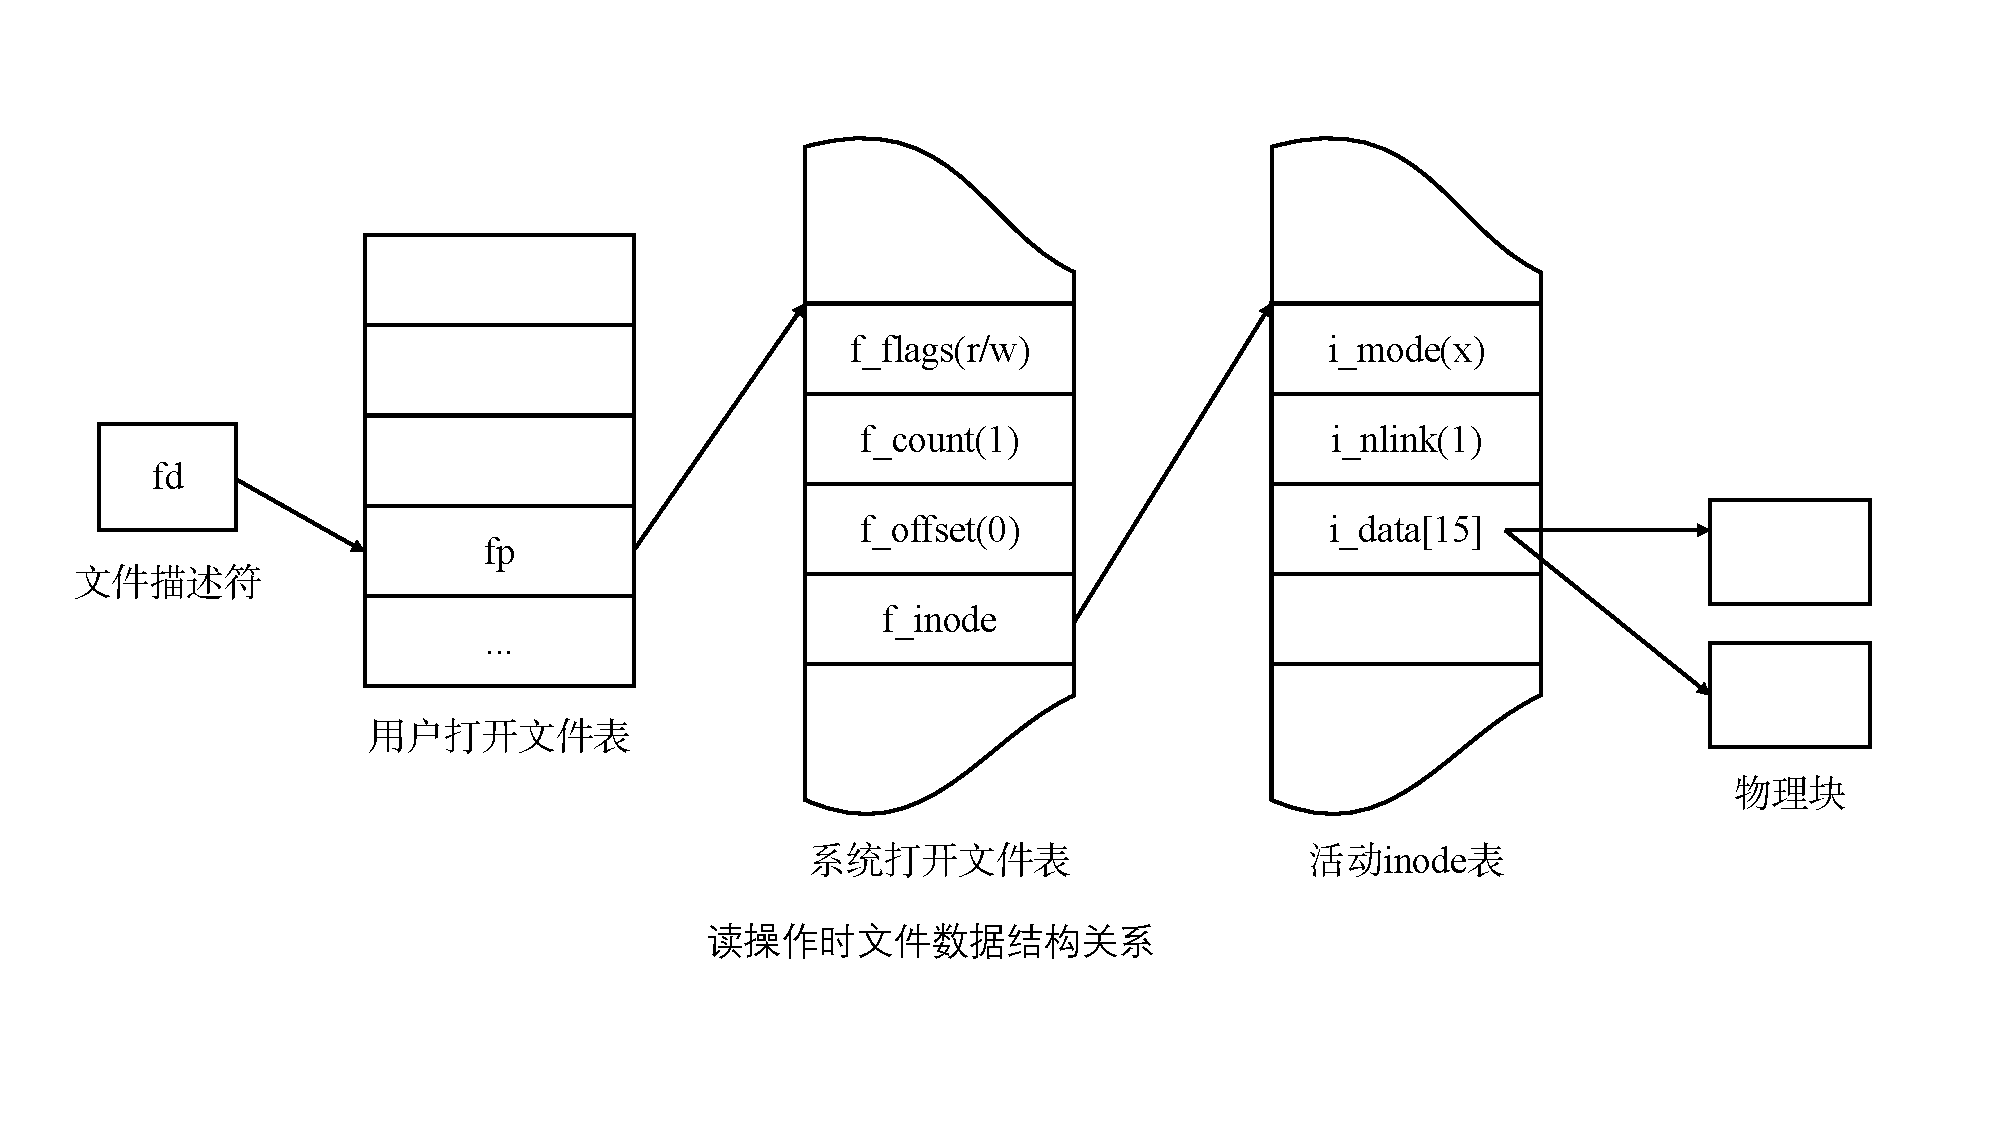
\includegraphics[width=0.8\textwidth]{img/读操作时文件数据结构关系}
	\end{figure}


	\subsubsection{文件的写入}
	\begin{lstlisting}[language=C,keywordstyle=\color{black}]
int nw;     	// 系统调用后实际写入的字节数
int fd;     	// 文件描述符
int count;  	// 要求传送的字符
char buf[];	 	// 数据传送的源地址
nw = write(fd, buf, count); // 把buf所指向的用户主存区中的信息,写入到文件中
	\end{lstlisting}


	\subsubsection{文件的随机存取}
	在文件初次“打开”时,文件的位移量f\_offset清空为零,以后的文件读写操作总是根据offset的当前值,顺序地读写文件

	为了支持文件的随机访问,提供系统调用lseek,它允许用户在读、写文件前,事先改变f\_offset的指向
	\begin{lstlisting}[language=C,keywordstyle=\color{black}]
long lseek;
long offset;
int whence, fd;
lseek (fd, offset, whence);		
	\end{lstlisting}
	文件描述字fd必须指向一个用读或写方式打开的文件
	\begin{itemize}
		\item 当whence是0时,则f\_offset被置为offset,
		\item 当whence是1时,则f\_offset被置为文件当前位置加上offset
	\end{itemize}


	\section{文件目录}
	\subsection{文件目录结构}

	\subsubsection{文件目录}
	文件目录是实现文件的“按名存取”的关键数据结构,目录结构一般是层次性的、非线性的,多维坐标可以通过一定方式降成一维坐标
	\begin{itemize}
		\item 文件目录需要永久保存,因此也组织成文件存放在磁盘上,称为目录文件
		\begin{itemize}
			\item 目录文件在需要时会调入内存
			\item 目录文件永不为空,至少包含两个目录项,即当前目录项“\verb|.|”和父目录项“\verb|..|”
		\end{itemize}
		\item 为了加快文件查找速度,通常将文件控制块汇集和组织在一起形成文件目录
		\begin{itemize}
			\item 文件控制块(File Control Block, FCB)是操作系统为每个文件建立的唯一数据结构,包含了全部的文件属性
			\begin{itemize}
				\item 文件由FCB和文件体组成,创建文件时,系统要同时创建FCB
			\end{itemize}
			\item 文件目录包含许多目录项,目录项具体记录两类实体,分别用于描述文件子目录和文件
		\end{itemize}
	\end{itemize}

	文件系统的基本功能之一就是负责文件目录的建立、维护和检索,要求编排的目录便于查找、防止冲突

	\subsubsection{Linux系统的文件目录建立方法}
	Linux系统的FCB中的文件名和其他管理信息分开,其他信息单独组成一个数据结构,称为索引节点inode,此索引节点在磁盘上的位置由inode号标识
	\begin{itemize}
		\item 文件系统中的每个文件都有一个磁盘inode与之对应,这些inode被集中存放于磁盘上的inode区
		\item FCB对于文件的作用,犹如PCB对于进程的作用,集中这个文件的所有相关信息,找到inode,就能获得此文件的必要信息
		\item 把FCB的主要内容与索引节点号分开,不仅能够加快目录检索速度,而且便于实现文件共享
	\end{itemize}

	\begin{figure}[H]
		\centering
		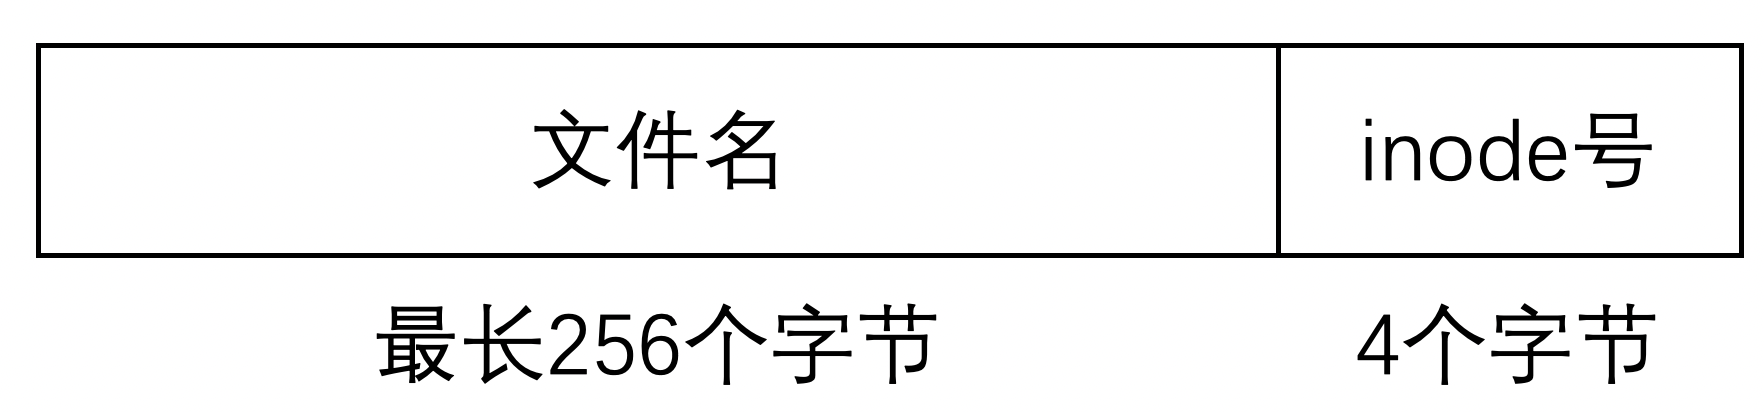
\includegraphics[width=0.45\textwidth]{img/Linux系统的FCB}
	\end{figure}

	\begin{lstlisting}[language=C,keywordstyle=\color{black}]
struct inode {
   unsigned long i_ino;                   /* inode号 */
   atomic_t i_counl;                      /* inode引用数 */
   kdev_t i_dev;                          /* inode所在设备 */
   loff_t i_size;                         /* inode所在设备 */
   nlink_t i_nlink;                       /* inode所在设备 */
   unsigned long i_blksize;               /* inode所在设备 */
   unsigned long i_block;                 /* inode所在设备 */
   struct inode_operations * i_op;        /* inode所在设备 */
   ...

   union {
      struct minix_inode_info minix_i;
      struct ext2_inode_infb ext2_i;
      ...
   }
}
	\end{lstlisting}

	由于磁盘inode记录文件的属性和相关信息,会被频繁访问,为此,在内存区开辟一张活动 inode 表,磁盘inode反映文件静态特性,活动inode反映文件动态特性
	\begin{itemize}
		\item 当访问某文件时,若在活动inode表中找不到其inode,就申请一个空闲活动inode,把磁盘inode内容复制给它,随之就可用来控制文件读写
		\item 当用户关闭文件时,活动inode的内容回写到对应的磁盘inode中,再释放活动inode以供它用
	\end{itemize}
	
	\subsubsection{一级目录结构与二级目录结构}
	一级目录结构:在操作系统中构造一张线性表,与每个文件的相关属性占用一个目录项,构成了一级目录结构
	\begin{itemize}
		\item 由于用户与文件众多,容易重名,不利于记忆
	\end{itemize}

	二级目录结构:一级目录结构的一种简单的扩展形式
	\begin{itemize}
		\item 第一级为主文件目录
		\begin{itemize}
			\item 用于管理所有用户文件目录
			\item 它的目录项登记了系统接受的用户的名字及该用户文件目录的地址
		\end{itemize}
		\item 第二级为用户的文件目录
		\begin{itemize}
			\item 为该用户的每个文件保存一个登记栏,其内容与一级目录的目录项相同
		\end{itemize}
		\item 每一用户只允许查看自己的文件目录
	\end{itemize}
	\begin{figure}[H]
		\centering
		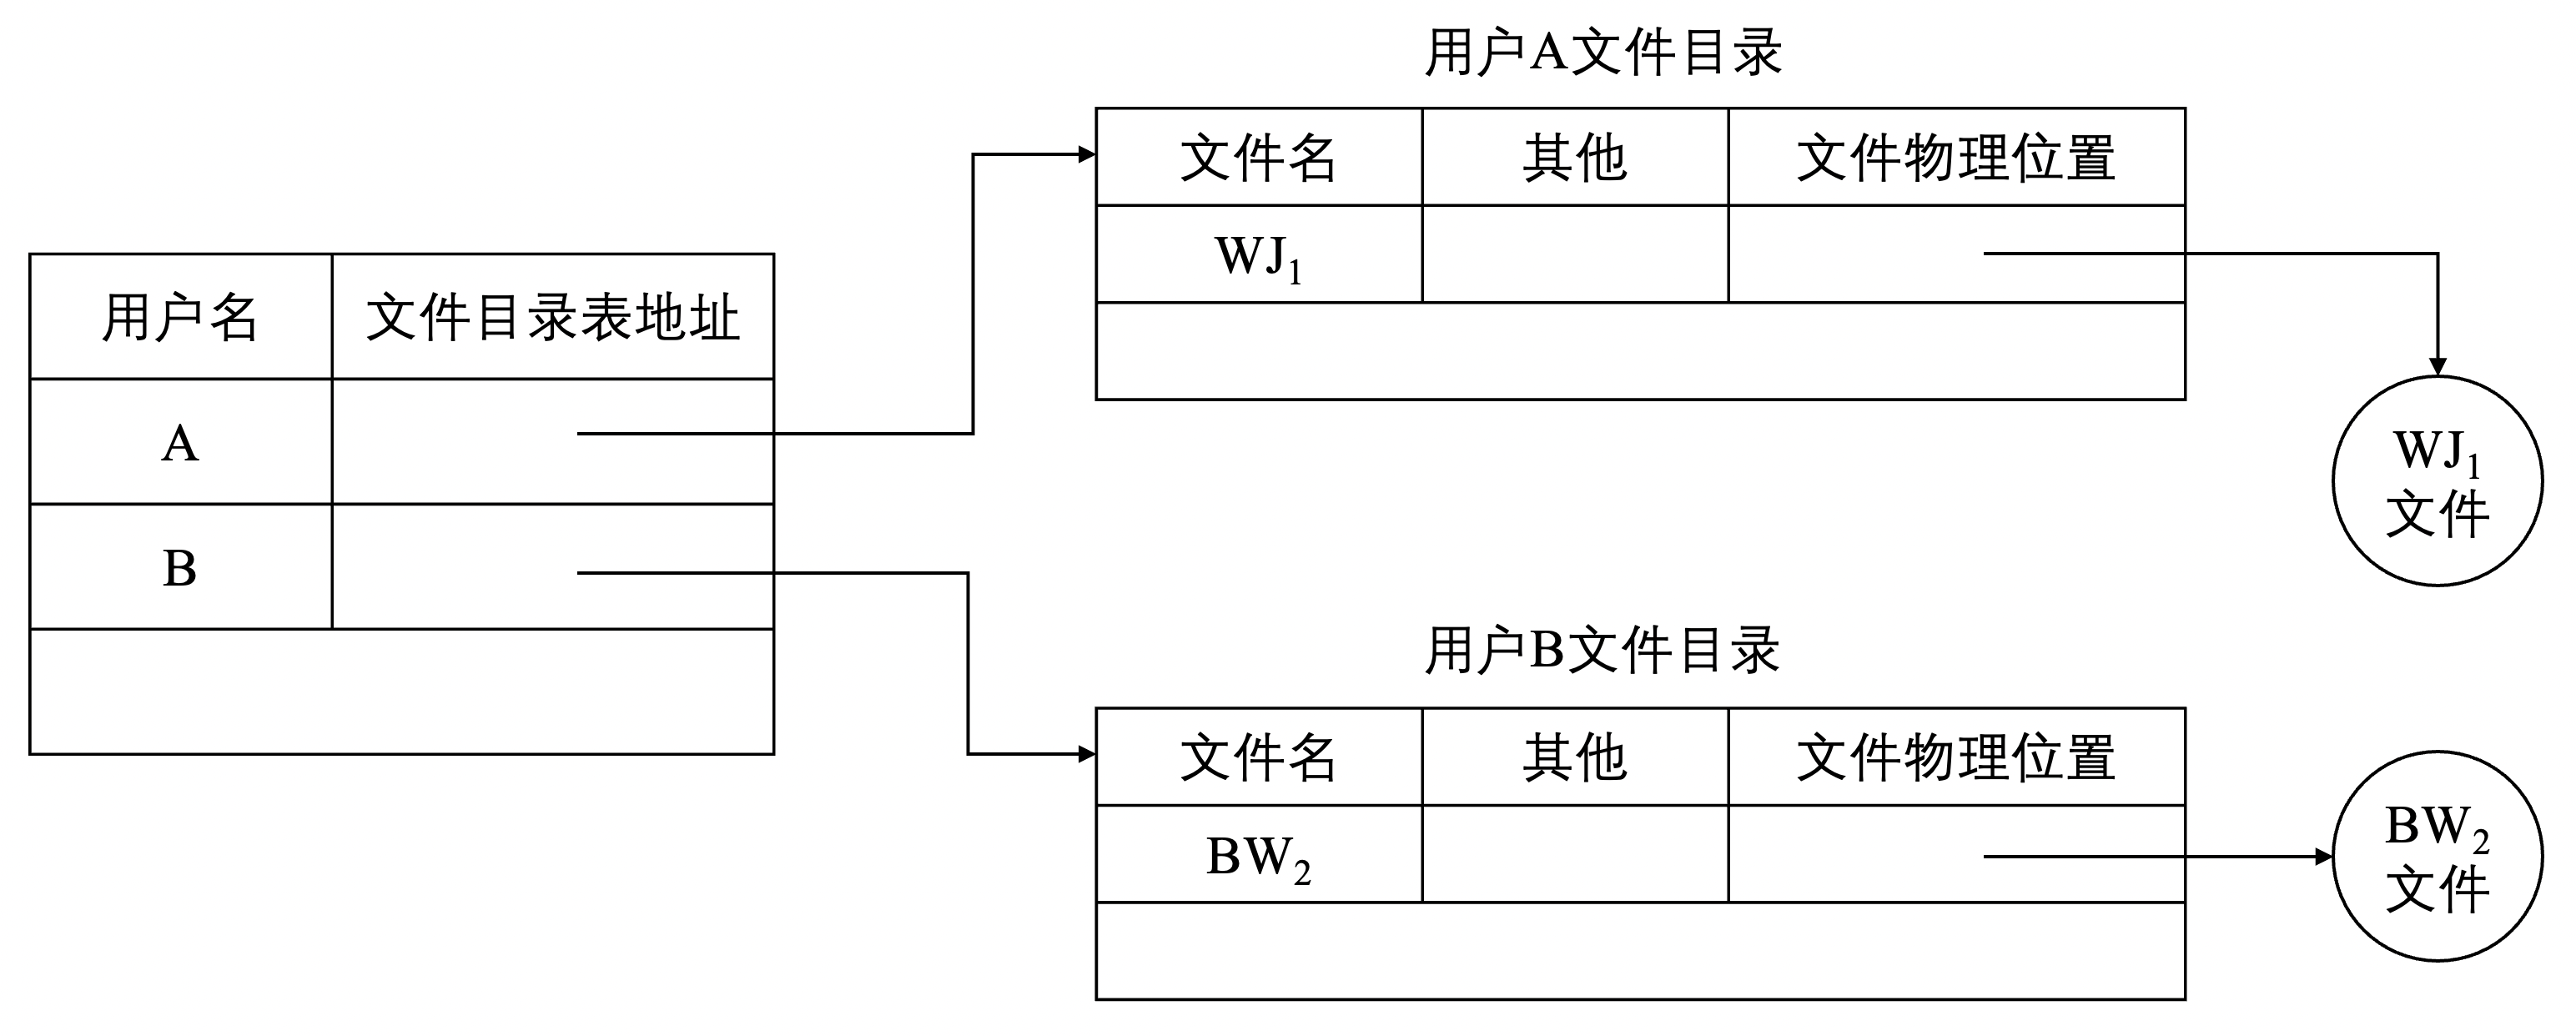
\includegraphics[width=0.98\textwidth]{img/5.3.1.2}
	\end{figure}

	二级目录结构的特点:
	\begin{itemize}
		\item 采用二级目录管理文件时,因为任何文件的存取都通过主文件目录,于是可以检查访问文件者的存取权限,避免一个用户未经授权就存取另一个用户的文件,使用户文件的私有性得到保证,实现了对文件的保密和保护
		\item 特别是不同用户具有同名文件时,由于各自有不同的用户文件目录而不会导致混乱
		\item 对于同一个用户而言,同样存在文件多、容易重名的问题
	\end{itemize}

	\subsubsection{层次目录结构}
	大多数文件系统支持多级层次目录结构,即根目录是唯一的,每一个目录项可以是下一级目录的说明,也可以是文件的说明,从而形成层次目录结构
	\begin{itemize}
		\item 层次目录结构通常采用树形目录结构,它是一棵倒向的有根树,树根是根目录,从根向下,每一个树分叉是一个子目录,而树叶是文件
	\end{itemize}

	\begin{figure}[H]
		\centering
		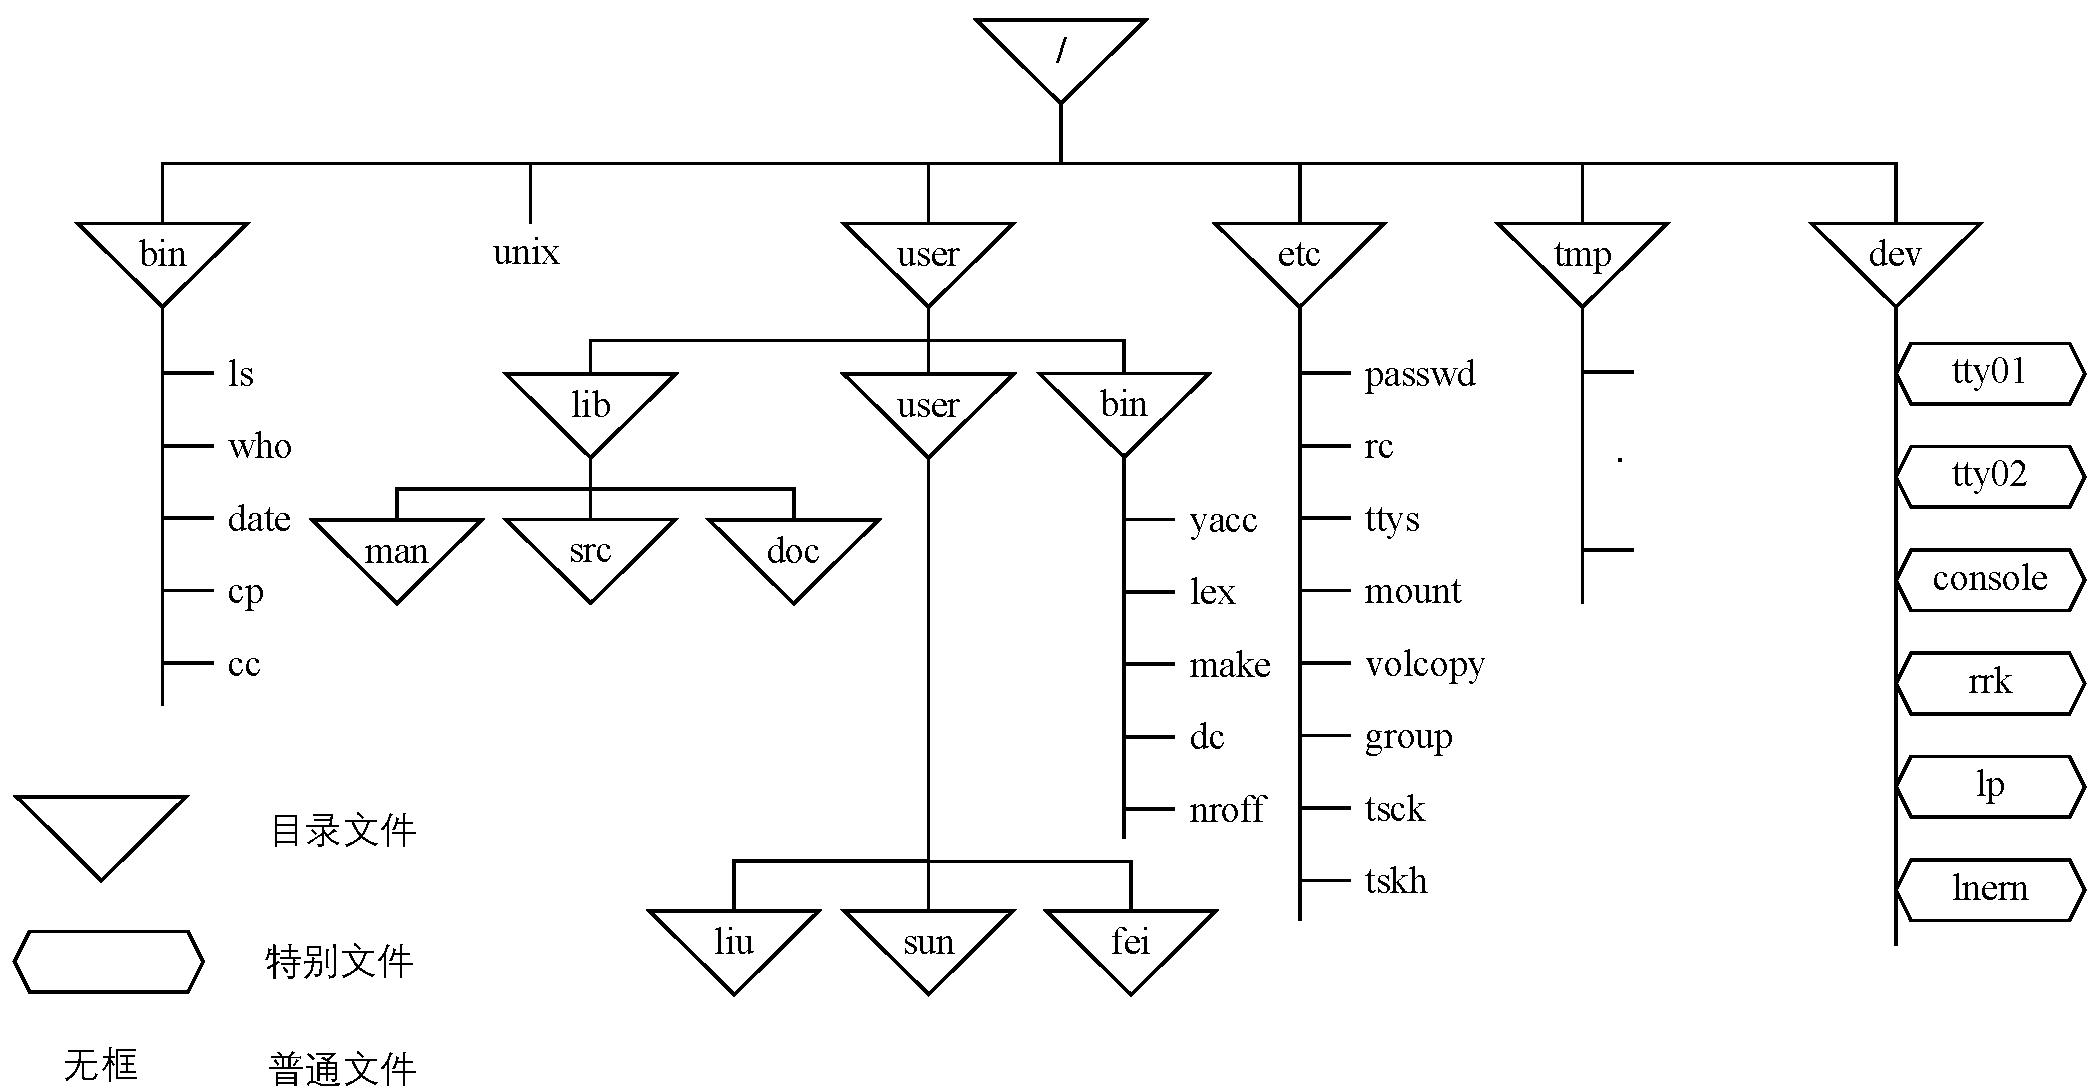
\includegraphics[width=0.98\textwidth]{img/5.3.1.3.1}
	\end{figure}

	树形目录结构的特点:
	\begin{itemize}
		\item 能较好地反映现实世界中具有层次关系的数据集合和较确切地反映系统内部文件的组织结构
		\item 不同文件可以重名,只要它们不位于同一末端的子目录中
		\item 易于规定不同层次或子树中文件的不同存取权限,便于文件的保护、保密和共享
	\end{itemize}

	树形目录结构中的文件定位:
	\begin{itemize}
		\item 在树形目录结构中,一个文件的全名包括从根目录开始到文件为止的通路上遇到的所有子目录路径,又称为路径名
		\item 各子目录名之间用正斜线“/”或反斜线“$\backslash$”分隔开
		\item 一个硬盘分区可以组织成一颗子树
		\begin{itemize}
			\item 每棵子树可以对应于一个逻辑盘符(Windows)
			\item 也可以把众多子树嫁接成一颗大树(UNIX)
		\end{itemize}
	\end{itemize}

	系统文件目录结构的实现
	\begin{itemize}
		\item 父目录包含子目录意味着包含一个指向子目录的文件目录项链接“\verb|.|”
		\item 子目录具有父目录也通过指向父目录的文件目录项来实现,即包含一项“\verb|..|”
		\item 对于文件系统的根目录,通常采用“\verb|.|”和“\verb|..|”都指向同一个文件目录项的方法实现
	\end{itemize}
	\begin{figure}[H]
		\centering
		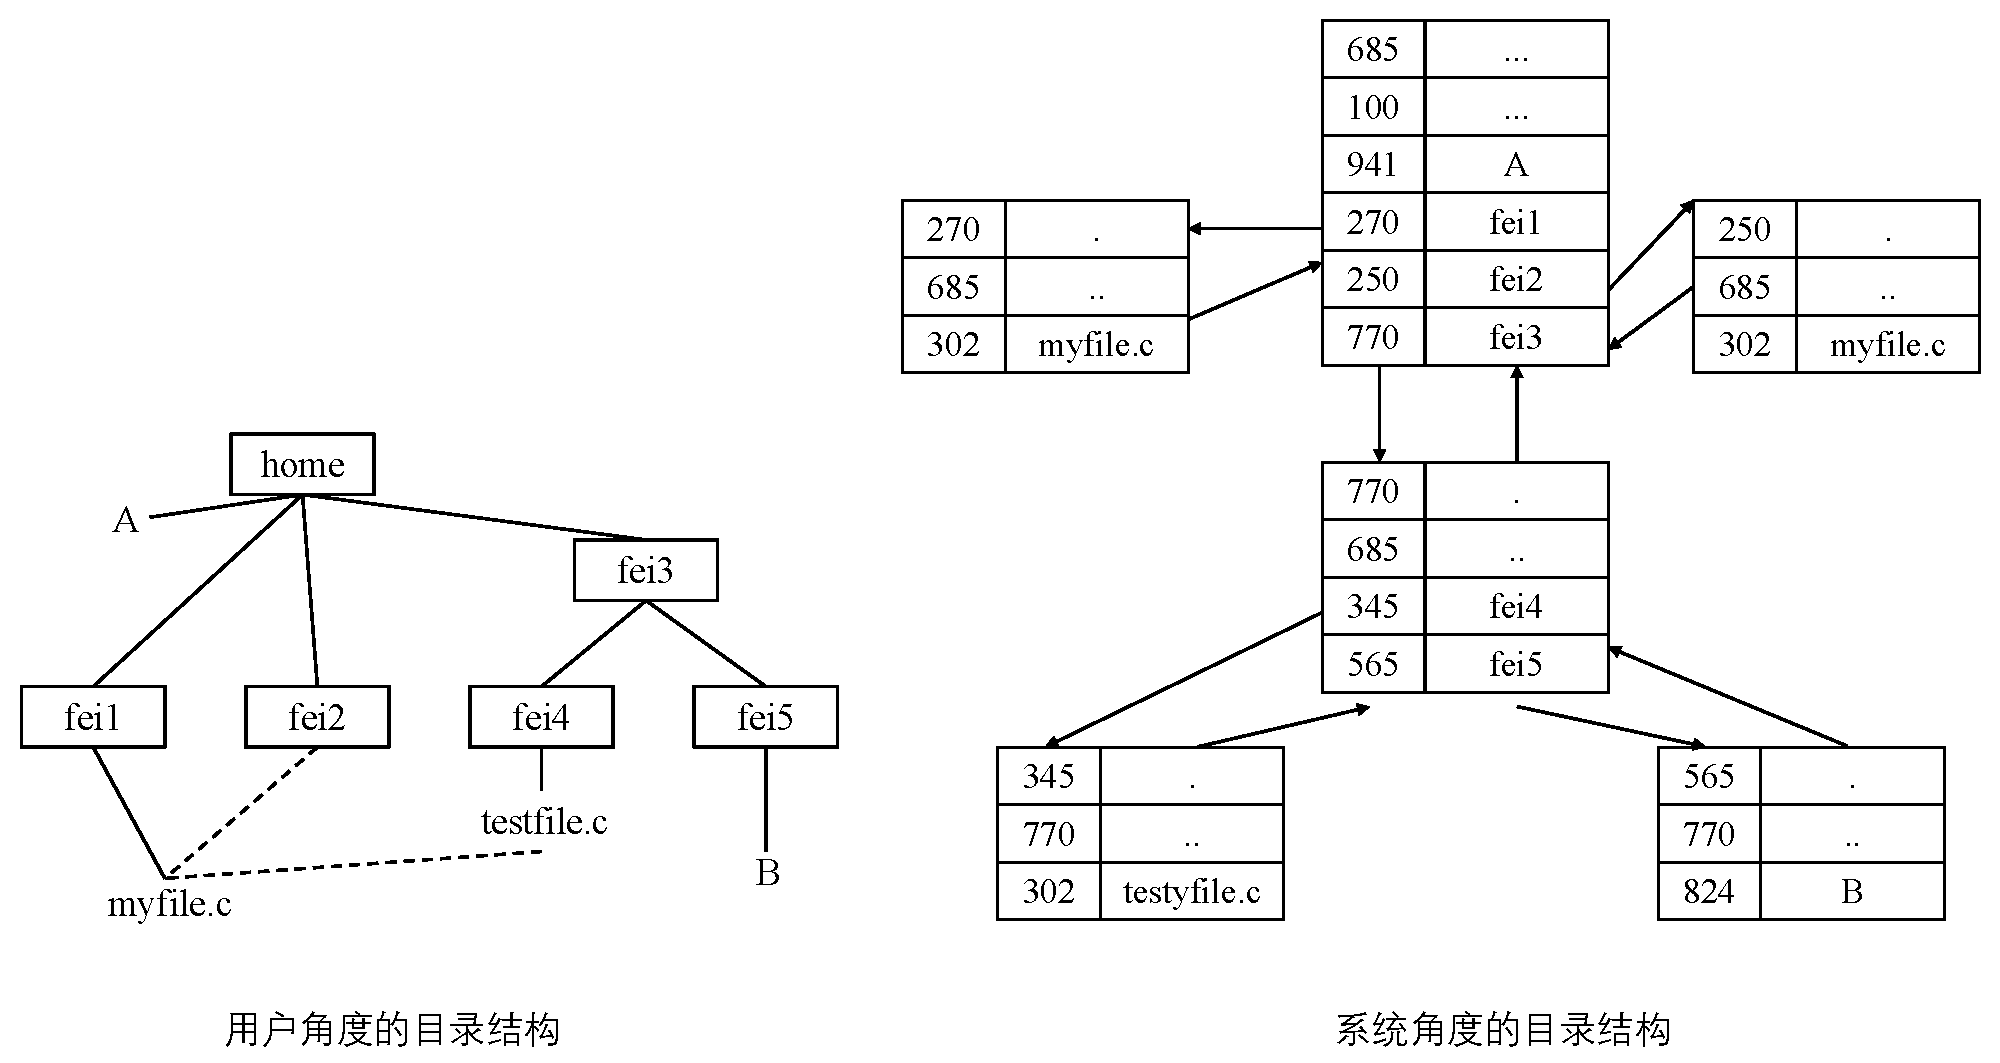
\includegraphics[width=0.98\textwidth]{img/5.3.1.3.2}
	\end{figure}

	\textbf{例:}假设应用进程要打开文件/home/fei1/myfile.c,文件系统的检索过程为
	\begin{enumerate}[label=\arabic*.]
		\item 首先,遇到根目录"/",它通常被存放在磁盘的固定盘块中,根据活动inode表中根目录的活动inode,把它作为当前工作索引节点并将其第一个物理块读入内存缓冲区
		\item 接着读入路径的第一个分量字符串home,文件系统对根目录的内容进行搜索,若找不到,则依次读入第二、第三个物理块,$\cdots$,进行比较,直至找到home的inode号
		\item 检查活动inode表
		\begin{itemize}
			\item 若找不到home的inode,为其分配一个活动inode,由于每个inode位于磁盘上已分配好的固定位置,可从磁盘home的inoe中装入其内容
			\item 否则,直接查找home的活动inode,通过属性查明home为子目录,经核对符合访问权限,把它作为当前工作索引节点,读入路径的第二个分量字符串fei1,父目录home对应的inode为685,从目录文件第一个物理块中可找到子目录fei1的inode为270
		\end{itemize}
		\item 类似地读入子目录fei1目录文件的物理块便能找到myfile.c的inode号为302,文件系统为此文件在活动inode表中分配一个活动inode,从myfile.c的磁盘inode中装入内容。中间任何一步出错都会返回错误码,由于路径名分析完毕,这时修改活动inode的有关内容,打开文件目录的查找操作到此结束
	\end{enumerate}

	\subsection{文件目录的管理}

	\subsubsection{文件的定位}
	文件查找是文件目录管理的重要工作,“按名存取”文件就是系统根据用户提供的文件路径名来搜索各级文件目录,找到该文件
	\begin{itemize}
		\item 可以从根目录查起(绝对路径名)
		\item 也可以从当前目录查起(相对路径名)
		\item 现代操作系统都设置有改变工作目录命令,即变更当前工作目录
	\end{itemize}

	\subsubsection{目录项的查找}
	搜索具体目录项时,可以采用顺序查找法,依次扫描文件目录中的目录项,将目录项中的名字与欲查找的文件名相比较

	可以采用一些优化办法加快查找目录的速度
	\begin{itemize}
		\item 若目录表项是按键的顺序编排,则可以采用“二分查找法”
		\item 或者采用“杂凑法”,把每个文件名经过变换函数变换成唯一的目录表表项
	\end{itemize}

	\subsubsection{活动文件表}
	系统可以为每个用户进程建立一张活动文件表
	\begin{itemize}
		\item 当用户使用一个文件之前,先通过“打开”操作,把该文件有关目录信息复制到指定主存区域,有关信息填入活动文件表,以建立用户进程和该文件索引的联系
		\item 当不再使用该文件时,使用“关闭”,切断用户进程和这个文件的联系,同时,若该目录已被修改过,则应更新辅存中对应的文件目录
	\end{itemize}

	\section{文件的共享、保护和保密}
	文件是计算机系统的重要资源,因此,要求文件系统具有保障文件安全的手段,提供文件保密的措施,有效地实现文件的共享
	\begin{itemize}
		\item \textbf{文件共享}是指不同用户共同使用某些文件
		\item \textbf{文件保护}是指防止文件被破坏
		\item \textbf{文件保密}则是指防止文件及其内容被其他用户窃取
	\end{itemize}

	\subsection{文件的共享}
	文件的共享是指不同进程共同使用用一个文件,这通常是计算机用户完成共同任务所必需的
	\begin{itemize}
		\item 文件共享带来许多好处:
		\begin{itemize}
			\item 减少用户大量重复性劳动
			\item 免除系统复制文件的工作
			\item 节省文件占用的存储空间
			\item 减少程序设计输入输出文件的次数
		\end{itemize}
		\item 文件共享的并发控制
		\begin{itemize}
			\item 在允许文件共享的系统中,操作系统应提供手段实现对共享文件的同步控制
			\item 多个进程可能同时存取一个文件,如果它们同时进行读操作,操作系统应对文件进行公用控制
			\item 如果有进程进行写操作,例如有两个进程,进程A要求修改文件,同时进程B要求读出同一文件中的数据,则操作系统必须提供同步控制机制,以保证文件数据的完整性
		\end{itemize}
		\item 文件的共享包含文件的静态共享、动态共享和符号链接共享等形式
	\end{itemize}

	\subsubsection{文件的静态共享}
	在Linux系统中,两个或多个进程可通过文件链接达到共享同一个文件的目的,无论进程是否存在,其文件的链接关系都存在,因此称为静态共享

	文件静态共享的系统调用
	\begin{lstlisting}[language=C,
		keywordstyle=\color{black}
	]
char* oldnamep;    // 指向已存在文件名的字符串的指针
char* newnamep;    // 指向文件别名的字符串的指针
link(oldnamep, newnamep);		
	\end{lstlisting}

	\begin{enumerate}[label=\arabic*.]
		\item 检索目录找到\verb|oldnamep|所指向文件的索引节点inode编号
		\item 再次检索目录找到\verb|newnamep|所指文件的父目录文件,并把已存在文件的索引节点inode编号与别名构成一个目录项,记入到该目录中去
		\item 把已存在文件索引节点inode的连接计数\verb|i_nlink|加1
	\end{enumerate}

	链接实际上是共享已存在文件的索引节点inode,完成链接的系统调用

	\textbf{例:}对于下列系统调用执行后
	\begin{lstlisting}[
		keywordstyle=\color{black},
	]
link("/home/fei1/myfile.c", "/home/fei2/myfile.c");
link("/home/fei1/myfile.c", "/home/fei3/fei4/testfile.c");
	\end{lstlisting}
	以下三个路径名指的是同一个文件
	\begin{lstlisting}[
		keywordstyle=\color{black},
	]
/home/fei2/myfile.c
/home/fei3/
fei4/testfile.c
	\end{lstlisting}


	文件解除链接调用形式为\ \verb|unlink (namep)|
	\begin{itemize}
		\item 解除链接与文件删除执行的是同一系统调用代码
		\item 删除文件是从文件主角度讲的,解除文件连接是从共享文件的其他用户角度讲的,都要删去目录项,把\verb|i_nlink|减1
		\item 不过,只有当\verb|i_nlink|减为0时,才真正删除文件
	\end{itemize}

	\subsubsection{文件的动态共享}
	文件动态共享是系统中不同的用户进程或同一用户的不同进程并发访问同一文件
	\begin{itemize}
		\item 这种共享关系只有当用户进程存在时才可能出现,一旦用户的进程消亡,其共享关系也就自动消失
		\item 在实现文件动态共享时,又分为两种情况:
		\begin{itemize}
			\item 共享位移指针的文件共享
			\item 不共享位移指针的文件共享
		\end{itemize}
	\end{itemize}

	\paragraph{共享位移指针的文件共享}~{}

	\begin{itemize}
		\item 同一用户父、子进程协同完成任务,使用同一读/写位移,同步地对文件进行操作
		\item 该位移指针宜放在相应文件的活动索引节点中。当用系统调用fork建立子进程时,父进程的PCB结构被复制到子进程的PCB结构中,使两个进程的打开文件表指向同一活动的索引节点,达到共享同一位移指针的目的
		\item 注意在下图中 \verb|f_count=2| 表示共享
	\end{itemize}

	\begin{figure}[H]
		\centering
		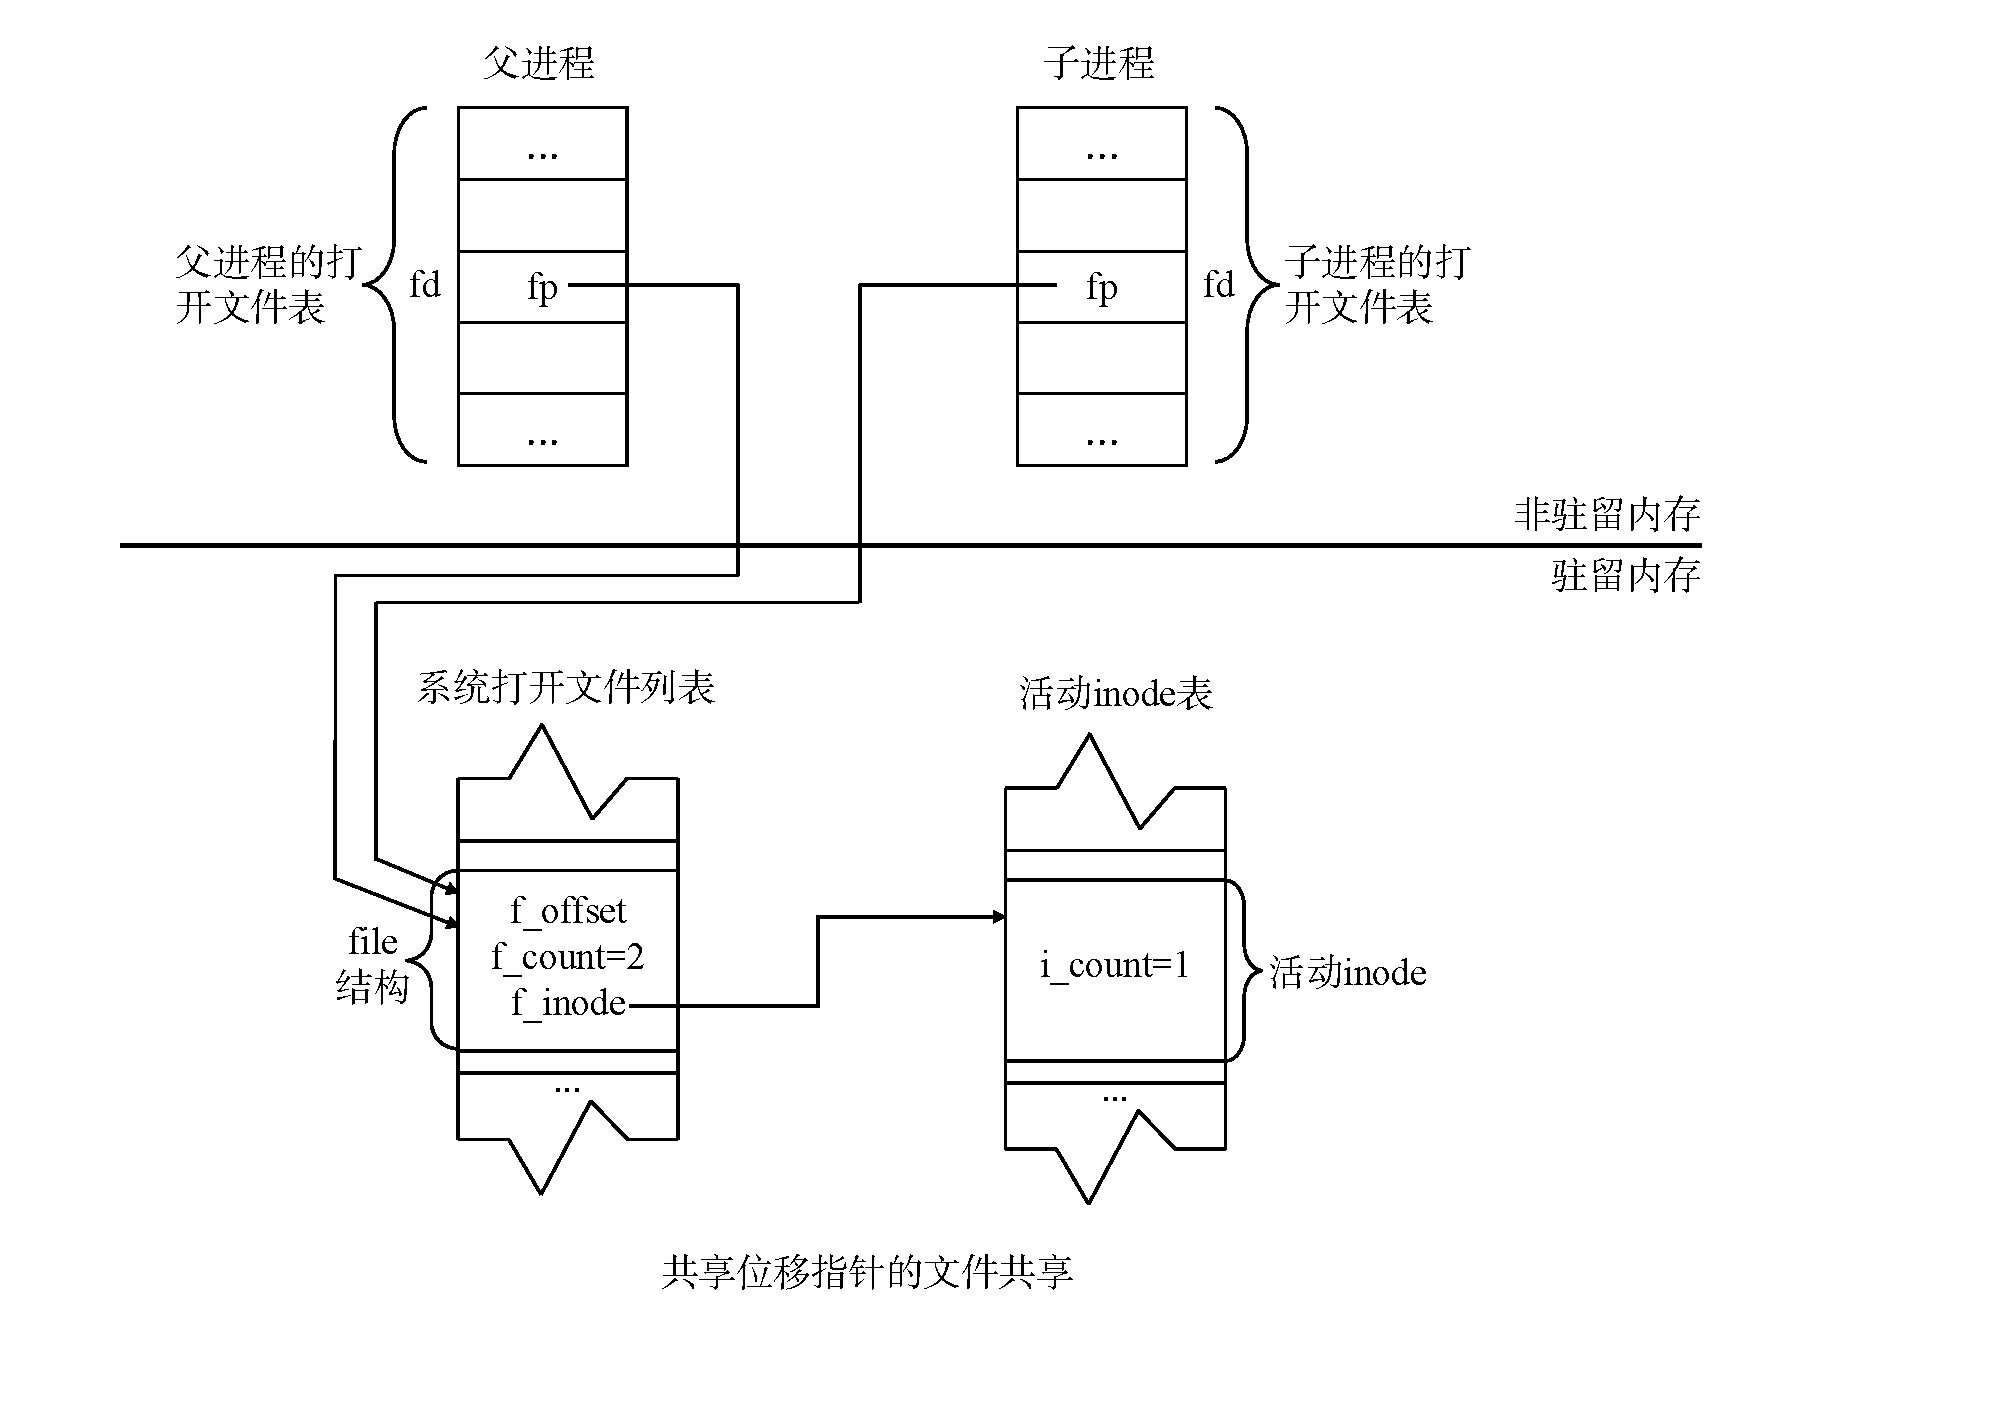
\includegraphics[width=0.8\textwidth]{img/5.4.1.2.1}
	\end{figure}
	
	\paragraph{不共享位移指针的文件共享}~{}

	\begin{figure}[H]
		\centering
		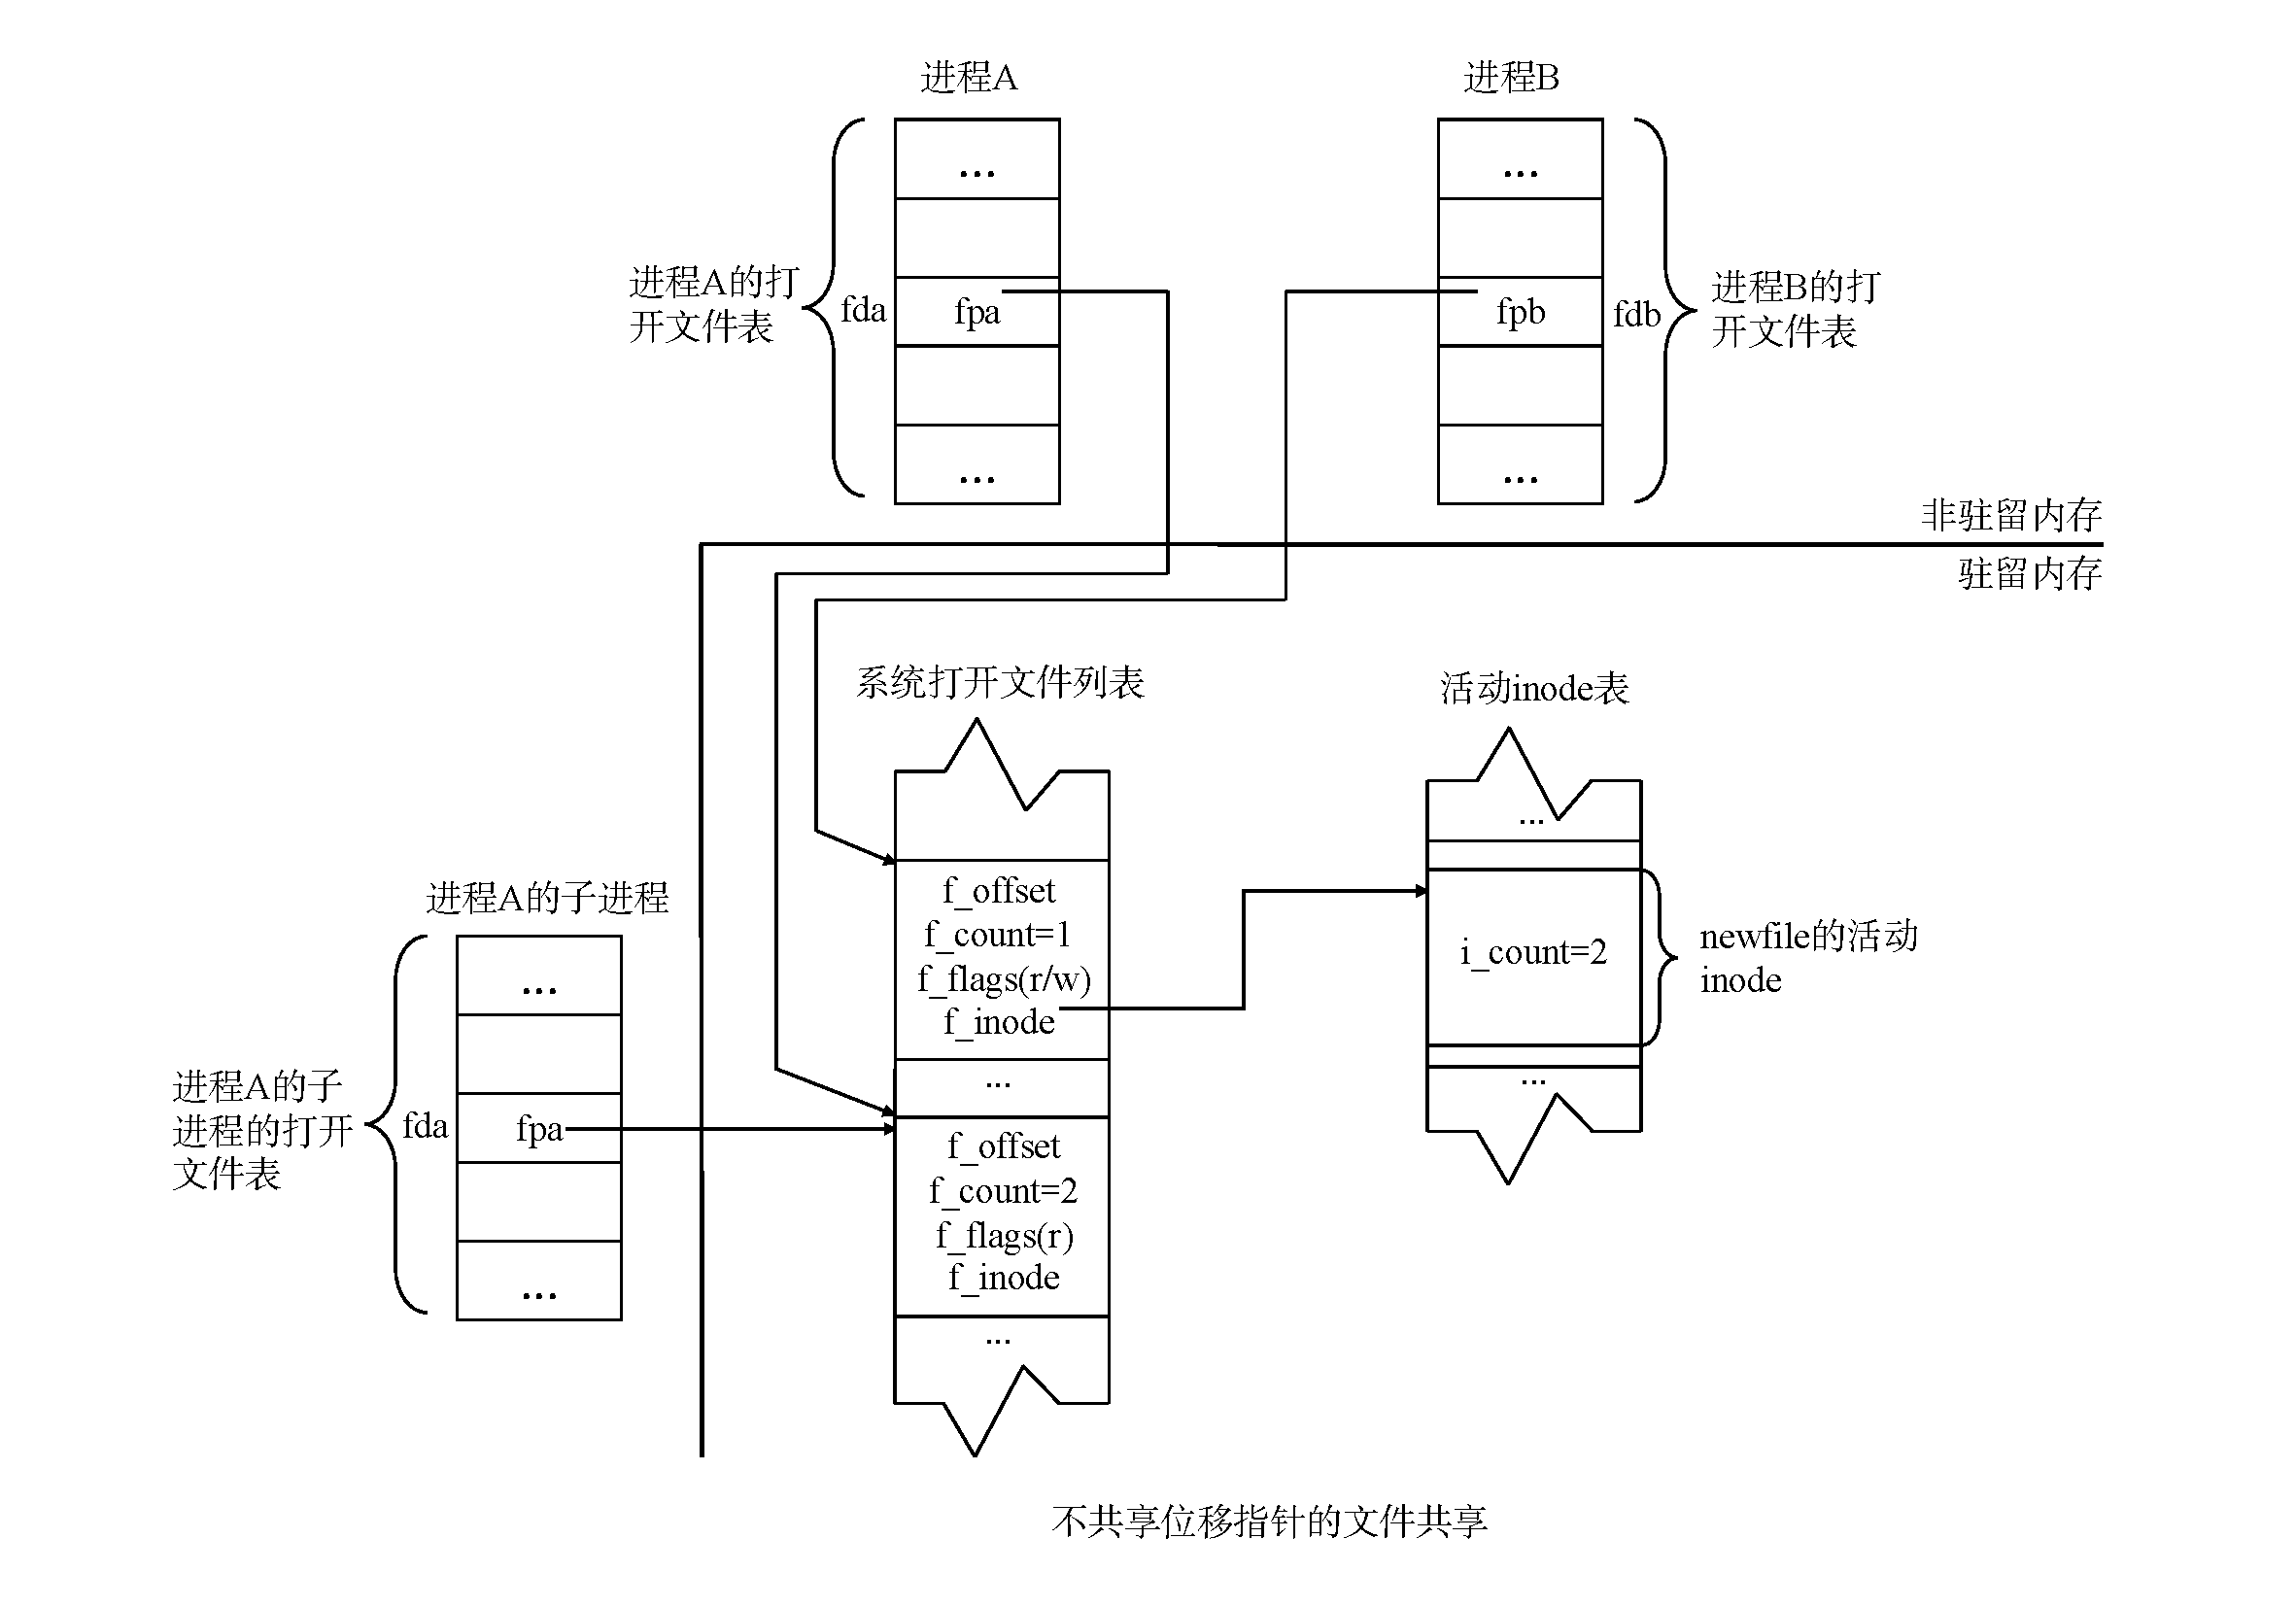
\includegraphics[width=0.9\textwidth]{img/5.4.1.2.2}
	\end{figure}

	\begin{itemize}
		\item 多用户共享文件,每个希望独立地读、写文件,这时不能只设置一个读写位移指针,须为每个用户进程分别设置一个读、写位移指针
		\item 位移指针应放在每个进程用户打开文件表的表目中
		\item 当一个进程读、写文件,并修改位移指针时,另一个进程的位移指针不会随之改变,从而,使两个进程能独立地访问同一文件
	\end{itemize}

	\subsubsection{文件的符号链接共享}
	在Linux文件系统中,每个文件对应一个索引结点,但是两个不同的磁盘或分区可能都含有相同索引结点编号所对应的文件,即在整合的目录树中,素引结点编号并不能唯一地标识一个文件,因而无法做到从不同文件系统生成指向同一个文件的链接
	\begin{itemize}
		\item 将文件名和自身的索引结点链接起来,称为硬链接
		\begin{itemize}
			\item 硬链接的优点是实现简单,访问速度快
			\item 但只能用于单个文件系统,却不能跨越文件系统,可用于文件共享但不能用于目录共享,可以通过软链接克服上述缺点
		\end{itemize}
		\item 软链接又称为符号链接,是只有文件名、不指向索引结点的链接,通过名称来引用文件
		\begin{itemize}
			\item 符号链接共享文件的实现思想:
			\begin{itemize}
				\item 用户A目录中形式为afile $\rightarrow$bfile,实现A的目录与B的文件的链接
				\item 其中只包含被链接文件bfile的路径名而不是它的inode号,而文件的拥有者才具有指向inode的指针
			\end{itemize}
			\item 当用户A要访问被符号链接的用户B的文件bfile,且要读“符号链接”类文件时,被操作系统截获,它将依据符号链接中的路径名去读文件,于是就能实现用户A使用文件名afile对用户B的文件bfile的共享
			\begin{itemize}
				\item 优点:能用于链接计算机系统中不同文件系统中的文件,可链接计算机网络中不同机器上的文件,此时,仅需提供文件所在机器地址和该机器中文件的路径名
				\item 缺点:搜索文件路径开销大,需要额外的空间查找存储路径
			\end{itemize}
		\end{itemize}
	\end{itemize}


	\subsection{文件的保密}
	文件保密是指文件及其内容不能被未经文件主授权的其他用户窃取,文件的保密措施包括以下几种:
	\begin{itemize}
		\item 隐蔽文件目录
		\item 设置口令
		\item 使用密码
	\end{itemize}

	\subsection{文件的保护}
	文件保护是指防止文件被破坏,操作系统必须提供文件保护机制,有效实现文件的完整性

	常用的文件保护办法有
	\begin{itemize}
		\item 文件副本
		\item 文件存取矩阵与文件存取表
		\item 文件属性
	\end{itemize}

	\subsubsection{文件的副本}
	文件系统必须要有防止硬软件故障,保存信息完整性的能力

	文件副本是解决这些故障的手段,文件副本技术主要有两种实现机制:
	\begin{itemize}
		\item 动态多副本技术
		\begin{itemize}
			\item 在多个介质上维持同一内容的文件,并且保证在更新内容时这些更新能够同步更新到不同的副本上
			\item 这种方法需要增加设备费用和系统负载,一般适用于容量较小且较为重要的文件
			\begin{itemize}
				\item 例如不需更新的系统文件及专用文件,当文件发生故障时只要切换到备用设备即可
			\end{itemize}
		\end{itemize}
		\item 转储、备份与恢复机制
		\begin{itemize}
			\item 文件转储:定时把文件复制转储到其它介质上,当某介质上出现故障时,复原转储文件
			\item 转储又可分成两种方式:
			\begin{itemize}
				\item 在一定时间间隔或一个单位处理结束时,系统自动复写更新过的文件和数据
				\item 每天或每周把文件信息全部复写一遍,需要时再通过装入转储文件来恢复系统,例如restore、backup等命令
			\end{itemize}
		\end{itemize}
	\end{itemize}

	\subsubsection{文件的存取控制矩阵}
	若系统为每个用户设置访问每个文件对象的存取属性,此时系统的全部用户对全部文件的存取属性就组成一个二维矩阵,称为存取控制矩阵
	$$\begin{pmatrix}
		a_{11} & a_{12} & ... & a_{1n} \\
		a_{21} & a_{22} & ... & a_{2n} \\
		. & . & ... & . \\
		a_{n1} & a_{n2} & ... & a_{nn} \\
	  \end{pmatrix}$$

	由于操作系统拥有很多用户和众多文件,存取控制矩阵一定是一个稀疏矩阵,因此可以将其简化为一张存取控制表
	\begin{itemize}
		\item 存取控制表是让每一个文件都附有一个表,它规定了不同用户对该文件的访问权限
		\item 存取控制表仅登记那些对文件拥有存取属性的部分
	\end{itemize}

	基于存取控制矩阵/表的文件保护
	\begin{itemize}
		\item 常见的存取属性:访问、读、写、执行、创建、删除、授权等等
		\item 系统通过查阅存取控制矩阵/表核对用户对文件的存取权限
		\item 文件属主可以使用grant、revoke等命令进行授权,甚至把授权权转授给他信任的用户
		\item 系统管理用户(超级用户)等同于文件属主权限,并获得对系统文件的授访问权权限
	\end{itemize}

	\subsubsection{文件属性}
	现代操作系统有一种广泛采用的简化文件保护方式
	\begin{itemize}
		\item 其思路是首先对用户进行分类,再针对每类用户规定文件属性
		\item 同时将存取属性也简化成文件属性,直接存储在文件子日录中
		\item 用户的分类可以是属主、合作者或其他,文件的属性可以分为读、写执行,在此情况下,就产生了9种不同的用户文件属性
		\item 在使用文件时,用户同时需要提出访问要求,系统将此要求与文件可访问权限进行比较以达到保证文件安全的目的
	\end{itemize}
	
	\begin{table}[H]
		\centering
		\begin{tabular}{|c|c|c|c|}
		\hline
			 & 读 & 写 & 执行 \\ \hline
		文件主  & 1 & 1 & 0  \\ \hline
		合作者  & 1 & 0 & 0  \\ \hline
		其他用户 & 1 & 0 & 0  \\ \hline
		\end{tabular}
	\end{table}

	为了方便系统控制用户的存取权限,UNIX系统专门设置了三条命令:\verb|chmod|、\verb|chown|\ 和\ \verb|cbgrp|
	\begin{itemize}
		\item \verb|chmod|\ 命令可以改变文件的读、写和执行属性
		\item \verb|chown|\ 命令用于变更文件属主
		\item \verb|chgrp|\ 命令用于变更用户伙伴
	\end{itemize}


	\section{文件系统的实现}

	\subsection{辅助空间管理}
	磁盘等大容量辅存空间被操作系统及许多用户共享,用户进程运行期间常常要建立和删除文件,操作系统应能自动管理和控制辅存空间

	随着用户文件不断建立和撤销,文件存储空间会出现许多“碎片”

	操作系统解决“碎片”的办法是整理“碎片”;在整理过程中,往往对文件重新组织,让其存放在连续存储区中

	磁盘文件空间分配采用两种办法
	\begin{itemize}
		\item 连续分配:
		\begin{itemize}
			\item 文件存放在辅存空间连续存储区中,在建立文件时,用户必须给出文件大小,然后查找到能满足的连续存储区供使用
			\item 优点是顺序访问时速度快,管理较为简单,但为了获得足够大的连续存储区,需定时进行“碎片”整理
		\end{itemize}
		\item 非连续分配:
		\begin{itemize}
			\item 一种方法是以块(扇区)为单位
			\begin{itemize}
				\item 扇区不一定要连续,同一文件的扇区按文件记录的逻辑次序用链指针连接或位示图
			\end{itemize}指示
			\item 另一种方法是以簇为单位
			\begin{itemize}
				\item 簇是由若干个连续扇区组成的分配单位
				\item 实质上是连续分配和非连续分配的结合
				\item 各个簇可以用链指针、索引表,位示图来管理
			\end{itemize}
			\item 优点是辅存空间管理效率高,便于文件动态增长和收缩
		\end{itemize}
	\end{itemize}

	\subsubsection{位示图法}
	磁盘空间通常使用固定大小的块,可方便地用位示图管理
	\begin{itemize}
		\item 用若干字节构成一张位示图,其中每一字位对应一个物理块,字位的次序与块的相对次序一致,字位为1表示相应块已占用,字位为0表示该块空闲
		\item 微型机操作系统VM/SP、Windows和MacOS等操作系统均使用这种技术管理文件存储空间
		\item 位示图法的主要优点是:
		\begin{itemize}
			\item 每个盘块仅需1个附加位,例如,若盘块长为1KB,位示图开销仅占0.012\%
			\item 可把位示图全部或大部分保存在主存,再配合现代机器都具有的位操作指令,实现高速物理块分配和去配
		\end{itemize}
	\end{itemize}



	\subsubsection{空闲块成组连接法}

	\begin{figure}[H]
		\centering
		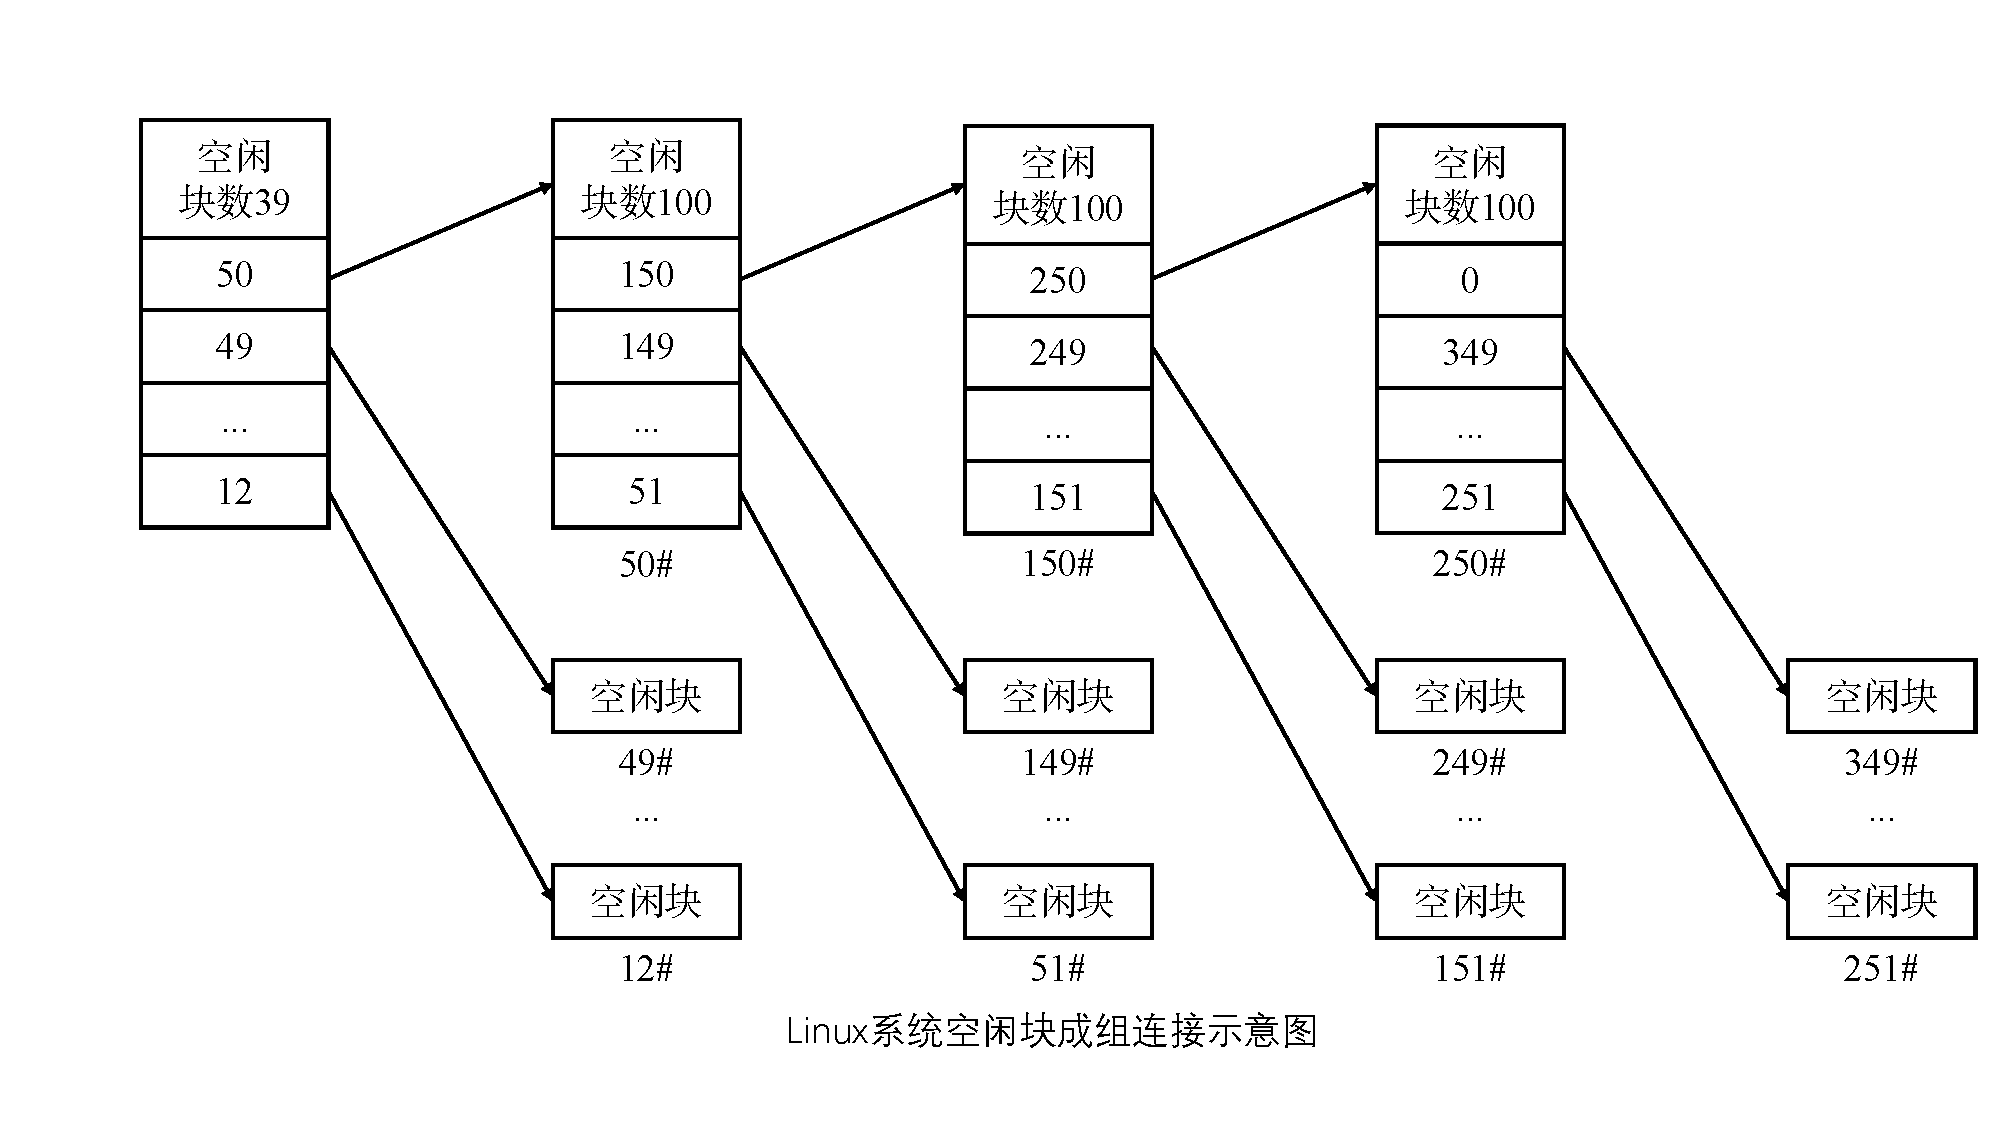
\includegraphics[width=0.9\textwidth]{img/5.6.1.2.1}
	\end{figure}

	上图给出Linux系统所采用的空闲块成组链接法,磁盘物理块长为1024B,为了方便讨论,假定文件卷启用时共有可用空闲块338块
	\begin{itemize}
		\item 目前空闲块分成4组,编号从12至349。前39块空闲块已在内存专用块中,剩余每100块划分成一组,每组中第一块(图中盘块号为50、68和188)登记下一组空闲盘块号和空闲块总数。需要注意的是,最后一组的第1项是0,作为结束标志,表明系统空闲盘块链已经结束。
		\item 操作系统启动时,将磁盘专用块复制到内存系统工作区中,访问内存专用块就可完成申请或释放空闲盘块的操作。
		\item 分配空闲磁盘块时,总是先把专用块中的空闲块计数减1,以它为指针找到专用块的相应表项,其内容就是要分配的空闲磁盘块号。
		\item 当空闲块计数减1后等于0时,专用块中仅剩1个磁盘块号,此时要取出表项中的磁盘块号(设为$i$),再把此盘块中所保存的下一组空闲磁盘块链接信息经缓冲区复制到内存专用块中,然后把当前磁盘块$i$分配出去。
		\item 释放存储块时,将磁盘块号记录在由专用块所指示的表项中,然后空闲块计数加1。若发现此表已满(达100项),则应把整个表的内容经缓冲区复制到下面要释放的磁盘块中,然后将释放块的块号写入专用块中的第一个位置,置空闲块计数为1。
		\item 搜索到磁盘块中的第1项是0时,系统应向操作员发出警告,表明空闲块已经用完。
		\item 需要注意的是,开始时空闲块是按序排列的,操作系统经过一段时间运行,文件系统中的空闲块号未必能保持连续,但只要符合分组及组间连接的原则,空闲块可按任意次序排列。事实上,经过若干次分配和释放操作后,空闲块物理块号必定不再按序排列。
	\end{itemize}

	\begin{figure}[H]
		\centering
		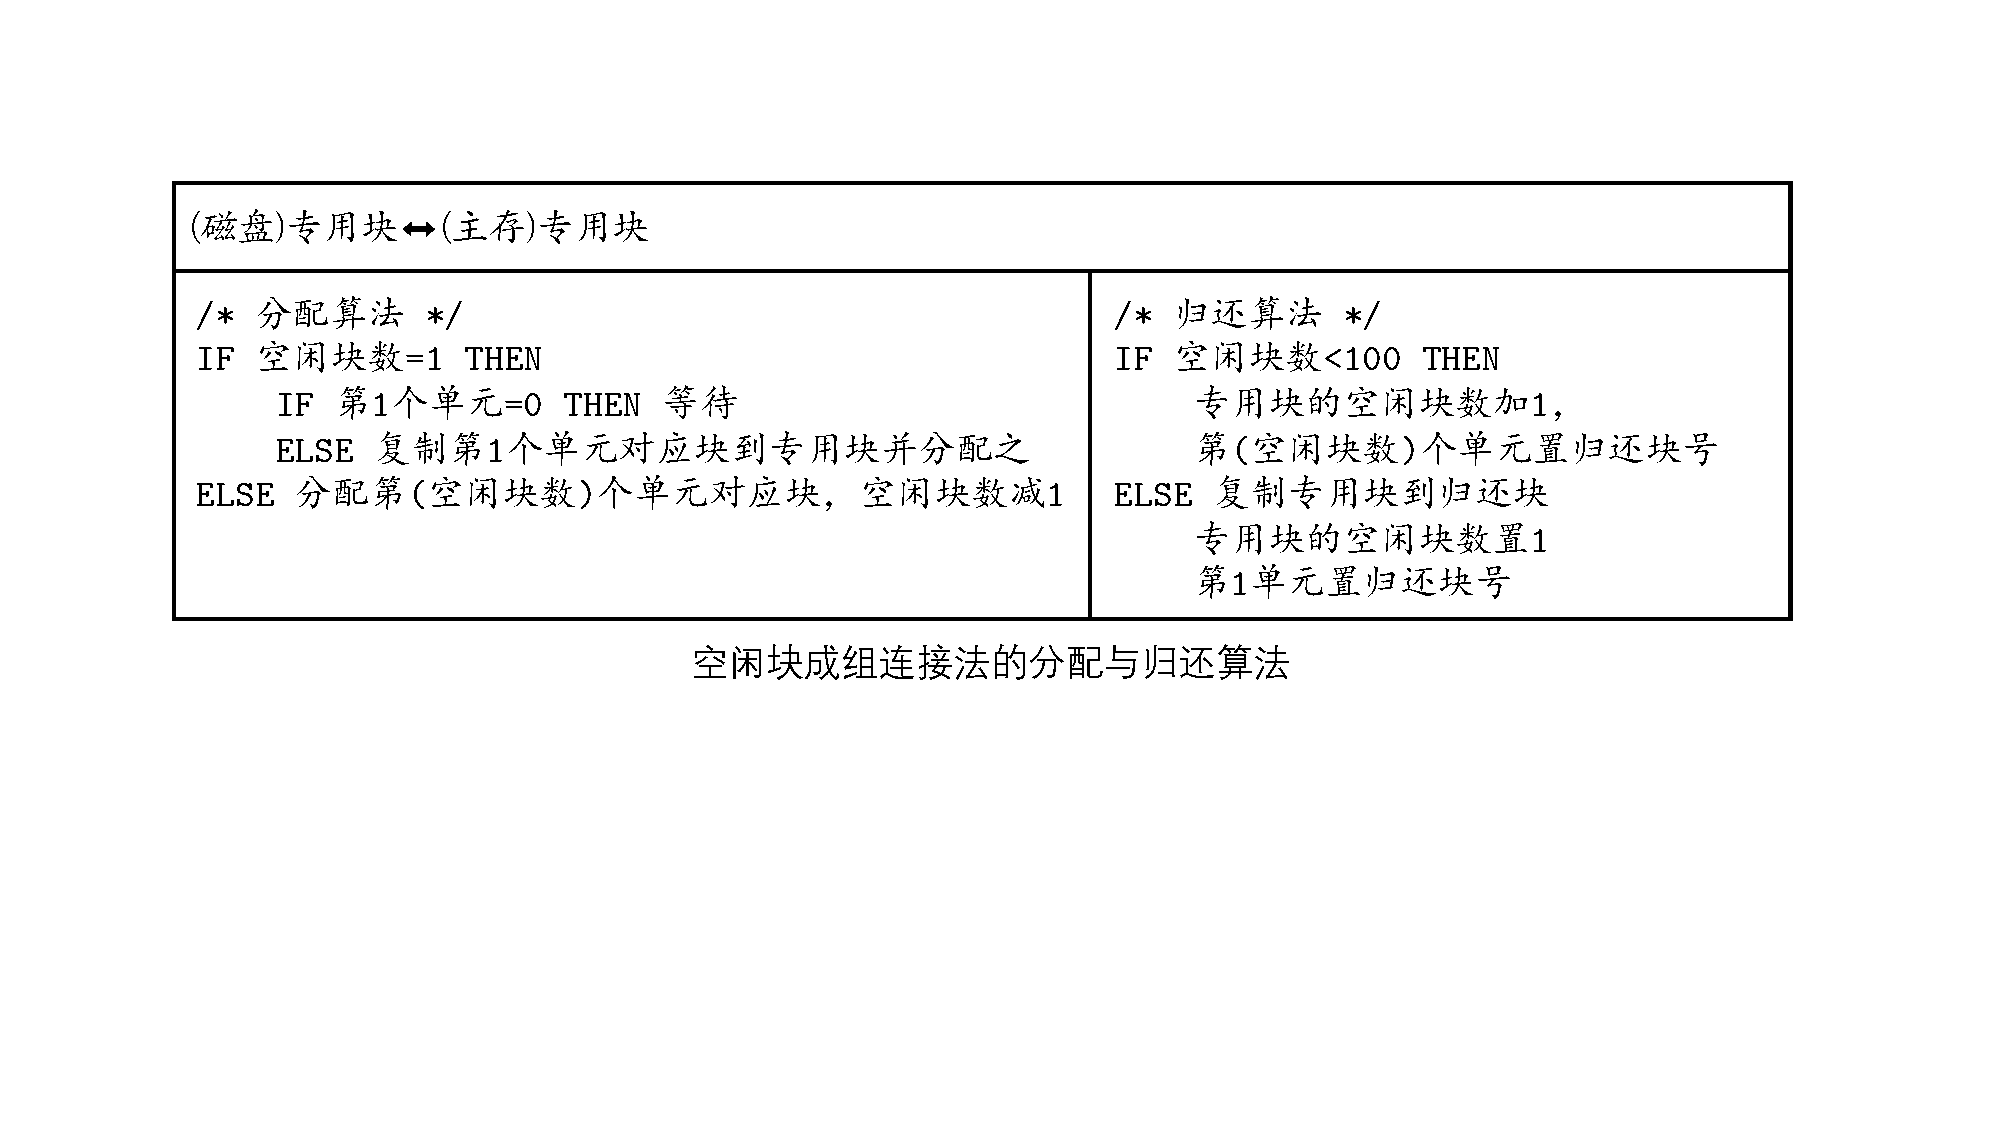
\includegraphics[width=0.9\textwidth]{img/5.6.1.2.2}
	\end{figure}

	\subsection{文件系统的实现层次}
	\begin{figure}[H]
		\centering
		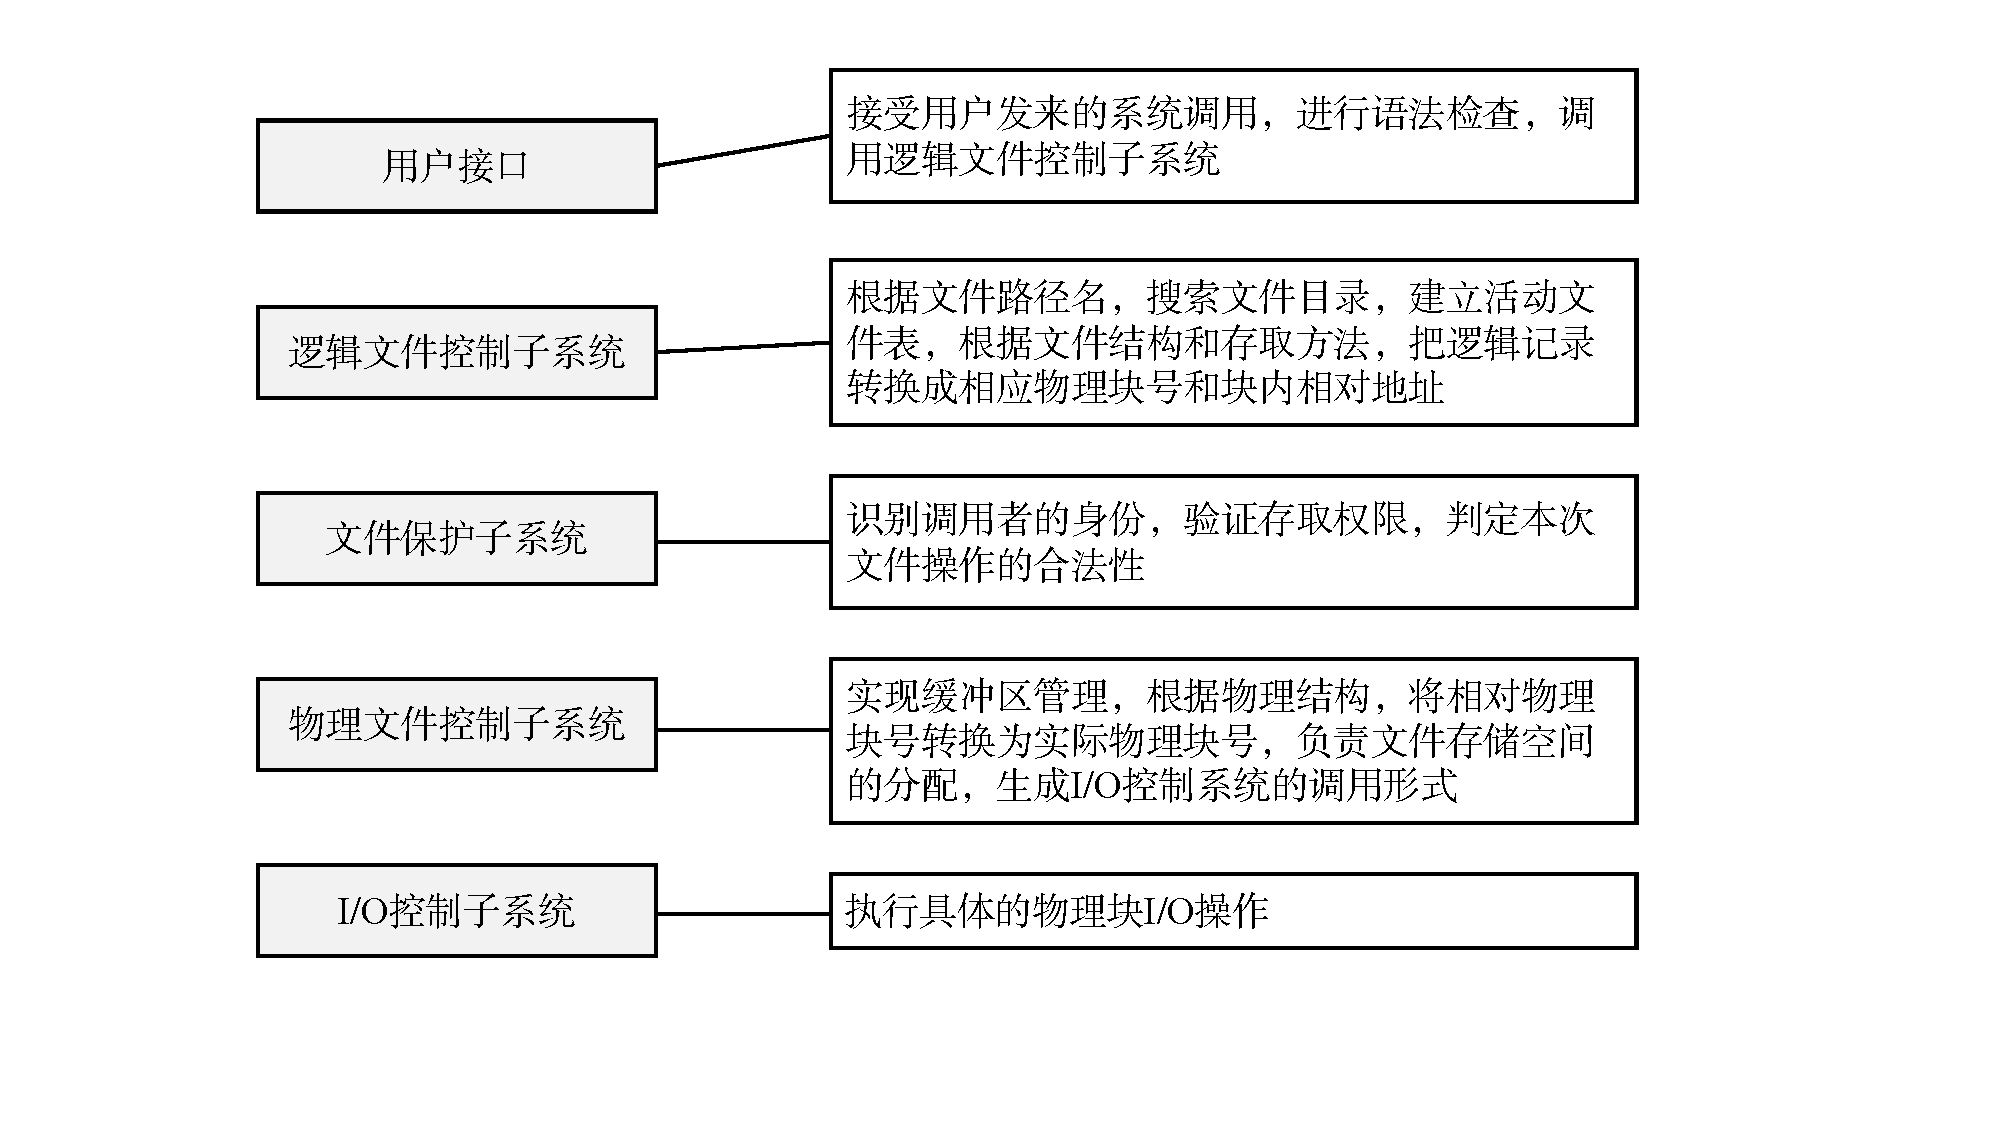
\includegraphics[width=0.75\textwidth]{img/5.6.2}
	\end{figure}


\end{document}


